% ============================================================================
% Appendix for PRL_attemption.tex
% Full mathematical details omitted from the 5-page PRL main text.
% ============================================================================
\documentclass[11pt]{article}

\usepackage{amsmath,amssymb,bm,geometry,graphicx,float,xcolor}
\geometry{margin=1in}

\title{EXperiments and Insights}
\author{Yuval Kochavi et al.}
\date{\today}

\begin{document}
\maketitle

\section{French2022}
This section is based on a comparison with the experimental data from Courtois et al. (2022) \cite{Courtois2022}. The work contains 2 different experiments, both with a with a SiO$_2$ tube coated with gold, one with density of $17.6 [\frac{mg}{cm^3}]$ and the second with $39.4 [\frac{mg}{cm^3}]$. The gold is 1.5 mm long and the tube diameter is 1.4 mm. Now note the that 17.6 foam is stongly transparent to radiation and therefore the diffusion approximation there is less valid, especially at early times. Moreover, the MFP is comparable to the tube diameter and so, an effective MFP correction will be needed here. The 39.4 foam is more opaque and therefore the diffusion approximation is more valid. Now one more thing we need to notice is that the breakout time of the heatwave was measured according to the inflaction point of the rising front. This could be calculated throw Fig 5a and 5b of the article~\cite{Courtois2022}, where we had to calculate in the inflaction point of the radiation tempratures for different lengthes, which accored at a fraction of 0.45-0.5 of the maximum temprature. And so when taking it to the forth order of the flux we get: 
\begin{equation}
    x_F^{'} = (1-0.5^4)^{\frac{4 + \alpha - \beta}{4}} x_F = (1-0.0625)^{\frac{4 + \alpha - \beta}{4}} x_F
\end{equation} 
But this had a really small effect on the final results. Note that when comparing to the results of $x_F$ we must take the beginning of the data to start from time 0, with value 0 at $t=0$. Another thing is that $T_{\mathrm{drive}}$ starts from time $0.3456\,\mathrm{ns}$, and so one must subtract this offset from the times of $T_D$.
Now for $n=0.6$ (MFP correction) and FT we get Fig.~\ref{fig:french22_front_position_gold17p6} for the front position of the SiO$_2$ gold-coating case (density 17.6): 
\begin{figure}[h!]
	\centering
	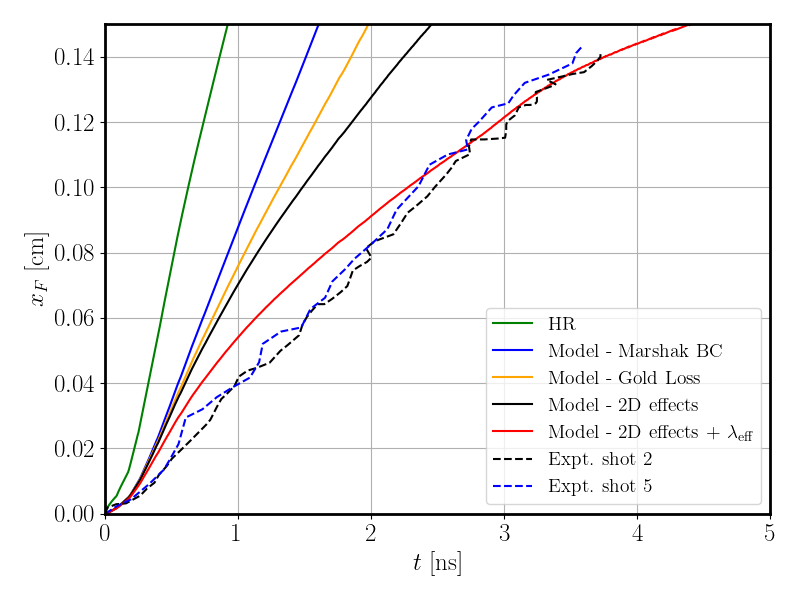
\includegraphics[width=0.45\textwidth]{figures_French22/front_position - gold coating (density 17.6).png}
	\caption{French2022: front position for the SiO$_2$ gold-coating case (density 17.6).}
	\label{fig:french22_front_position_gold17p6}
\end{figure}

Fig.~\ref{fig:french22_curvature_and_t4}a for the curvature comparison at $z=1.5\,\mathrm{mm}$ where we subtract a constant offset of $0.15 ns\,\mathrm{ns}$ from $t_{\mathrm{arr}}$ as some kind of average between 0 and 0.3456 ns, and Fig.~\ref{fig:french22_curvature_and_t4}b for the spatial $T^4$ heatmap at $t=4.5\,\mathrm{ns}$.
\begin{figure}[h!]
	\centering
	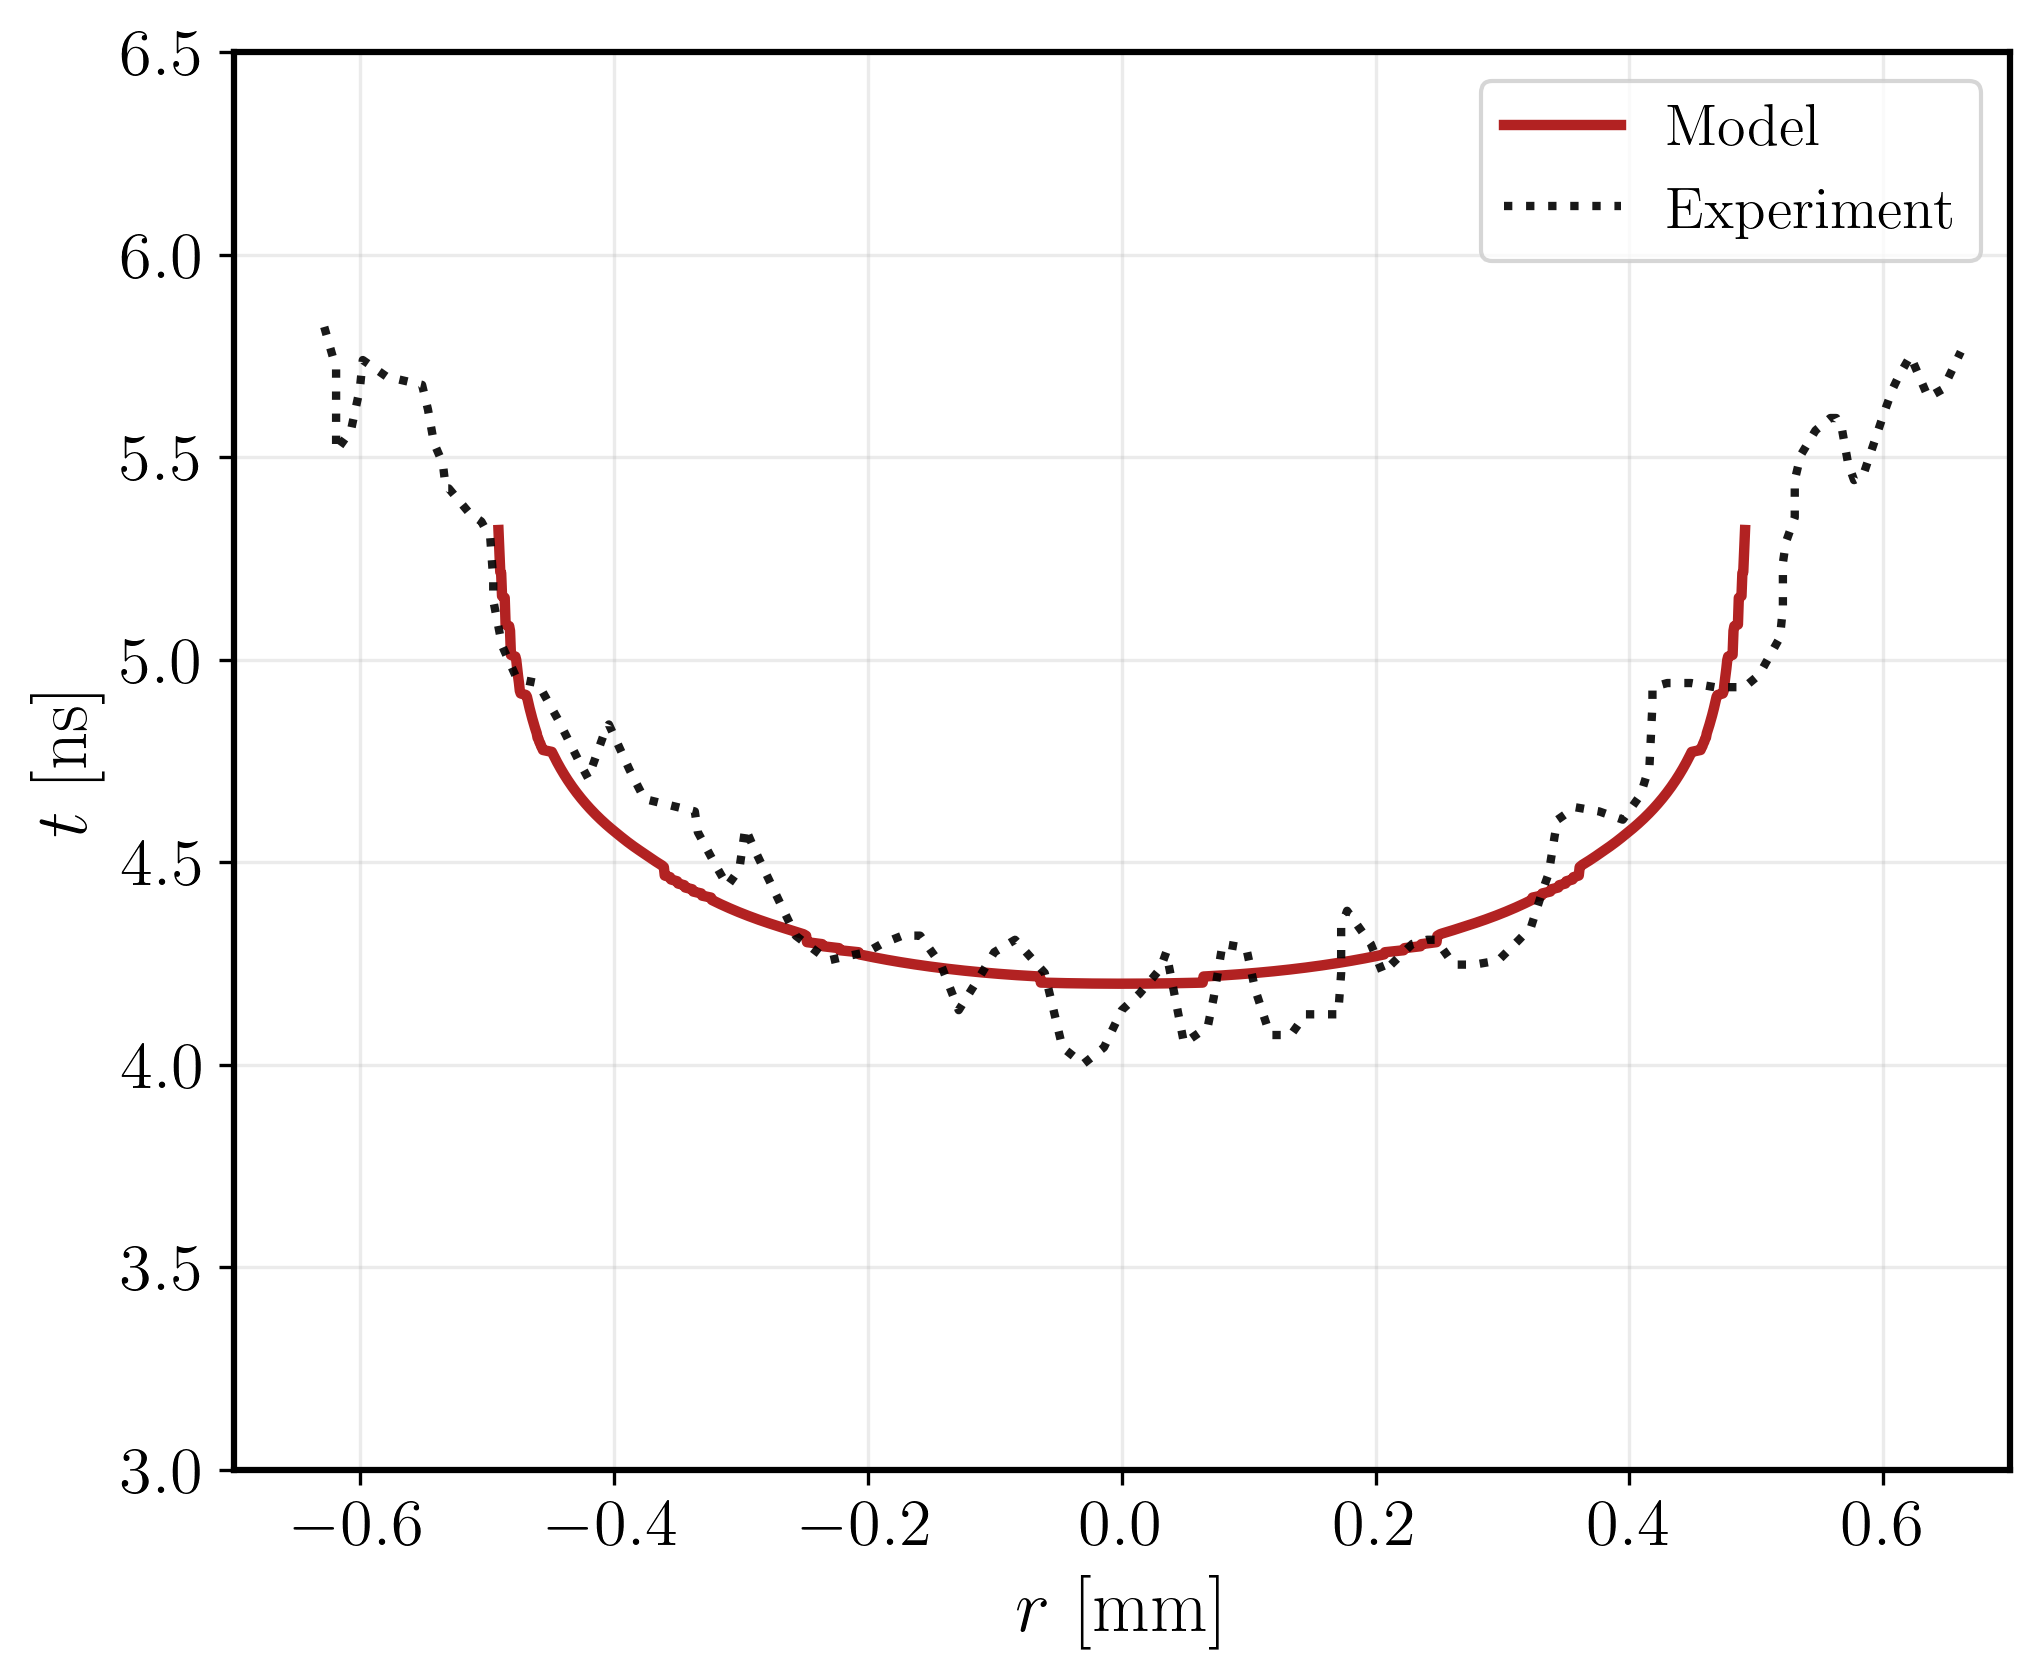
\includegraphics[width=0.48\textwidth]{figures_French22/curvature_comparison_1.5mm.png}
	\hfill
	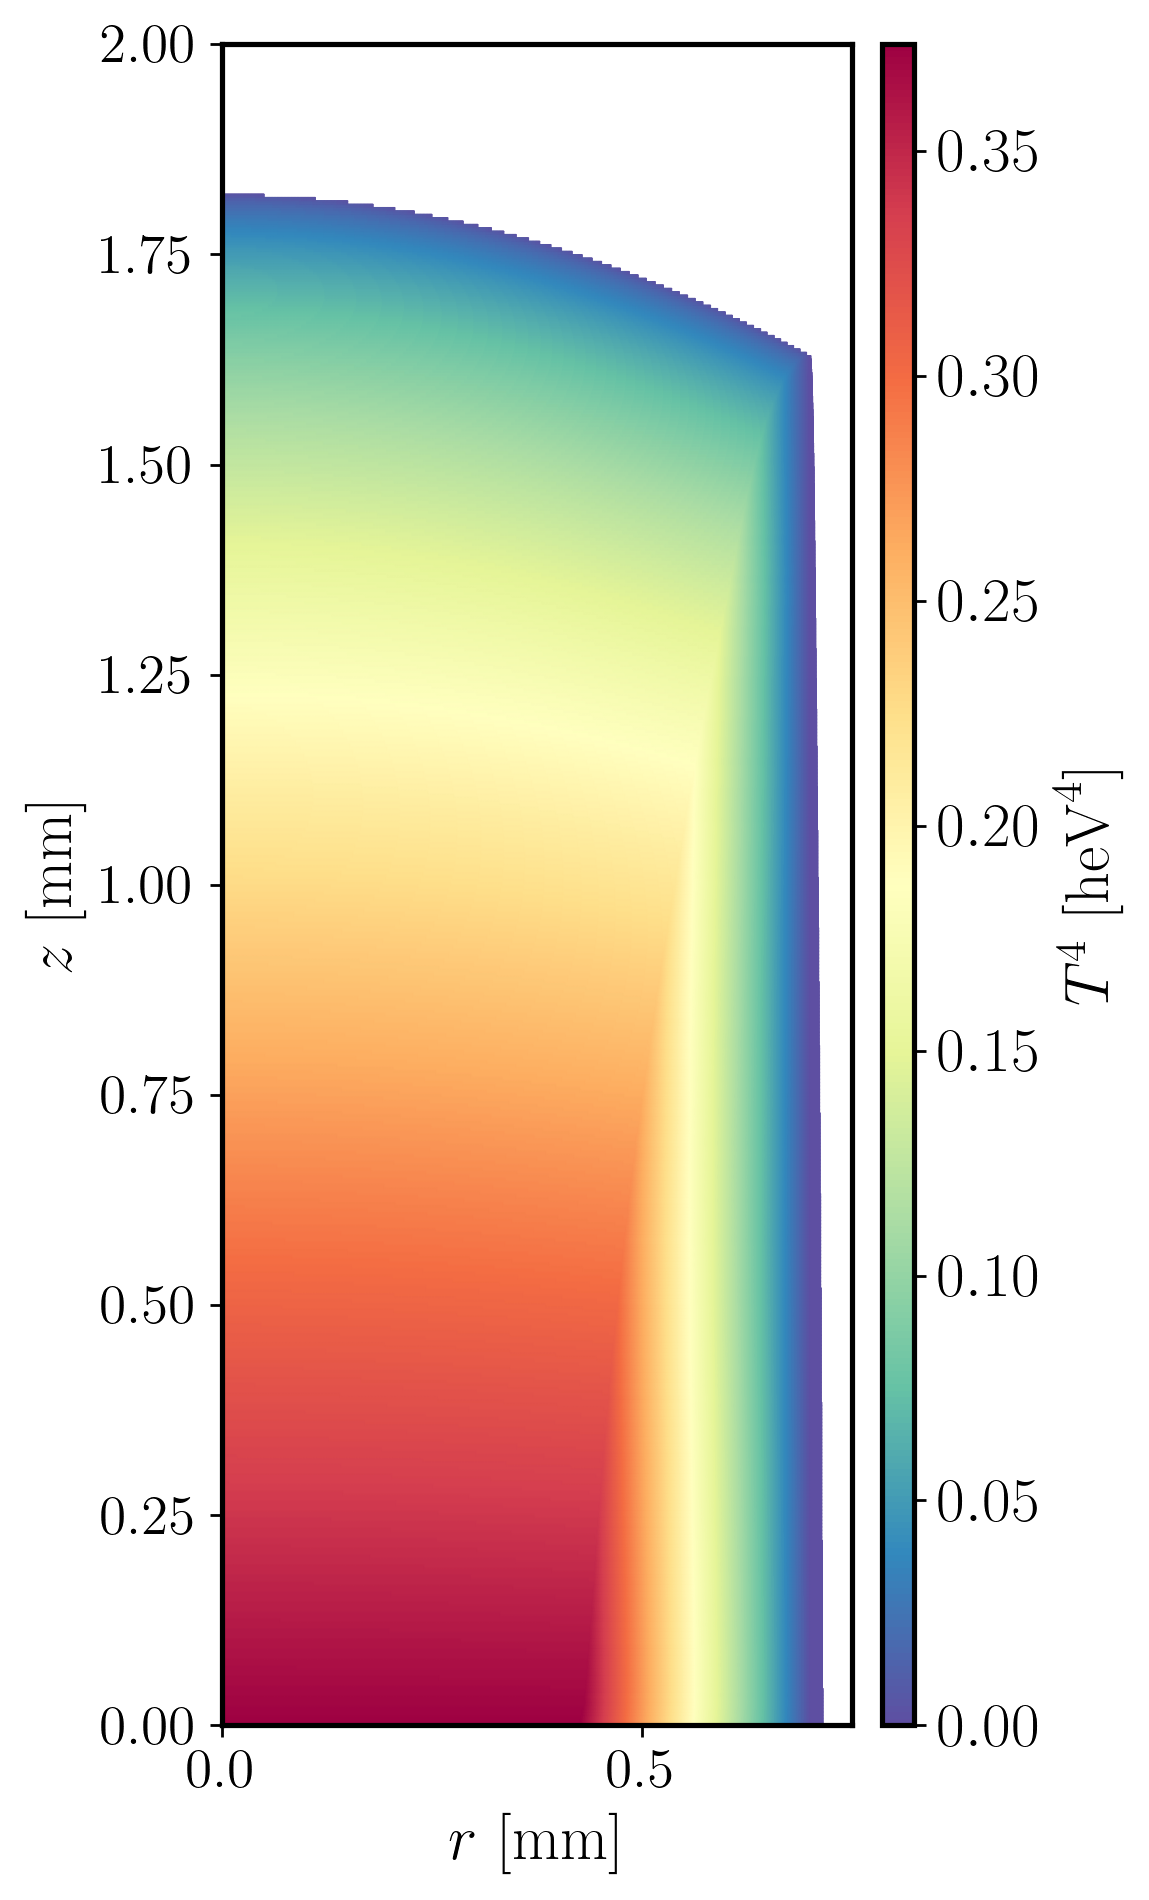
\includegraphics[width=0.28\textwidth]{figures_French22/T4_spatial_heatmap_4.5ns.png}
	\caption{French2022: comparison of model and experimental curvature at $z=1.5\,\mathrm{mm}$ (left), and spatial $T^4$ heatmap at $t=4.5\,\mathrm{ns}$ (right).}
	\label{fig:french22_curvature_and_t4}
\end{figure}

The MFP along time graph will be (with the optical depth $\tau$) Fig.~\ref{fig:french22_mfp_with_tau}: 
\begin{figure}[h!]
	\centering
	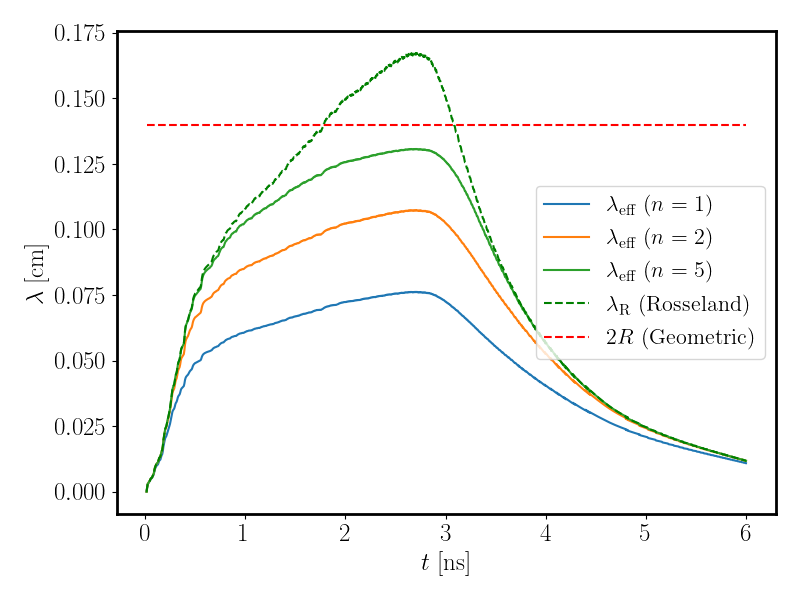
\includegraphics[width=0.45\textwidth]{figures_French22/lambda_eff_vs_time.png}
	\caption{effective mean free path $\lambda_{\mathrm{eff}}$ and optical depth $\tau$ as functions of time - 17.6 mg/cm$^3$.}
	\label{fig:french22_mfp_with_tau}
\end{figure}

Now for the 39.4 mg/cm$^3$ case we get Fig.~\ref{fig:french22_front_position_gold39p4} for the front position when using $n=1$ and FT:
\begin{figure}[h!]
    \centering
    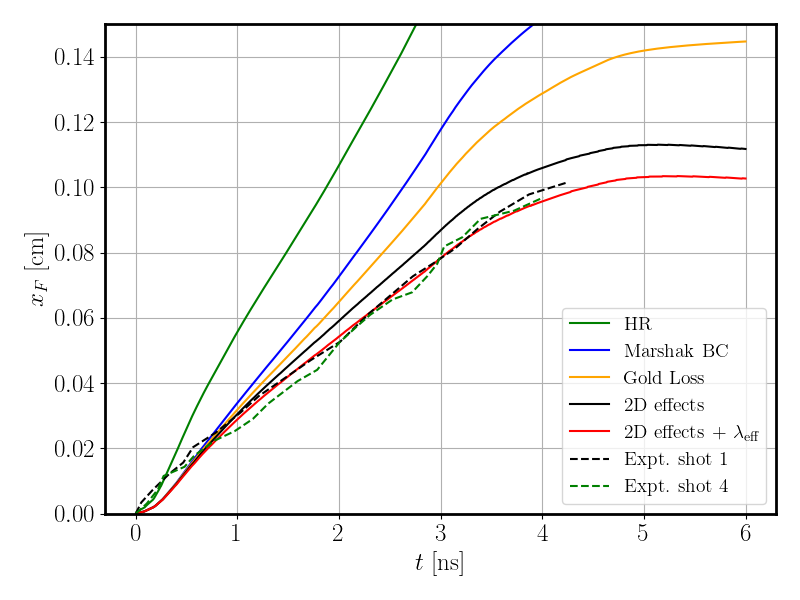
\includegraphics[width=0.45\textwidth]{figures_French22/front_position - gold coating (density 39.4).png}
    \caption{French2022: front position for the SiO$_2$ gold-coating case (density 39.4).}
    \label{fig:french22_front_position_gold39p4}
\end{figure}
\vspace{9em}
The MFP along time graph will be (with the optical depth $\tau$) Fig.~\ref{fig:french22_mfp_with_tau_39p4}:
\begin{figure}[h!]
    \centering
    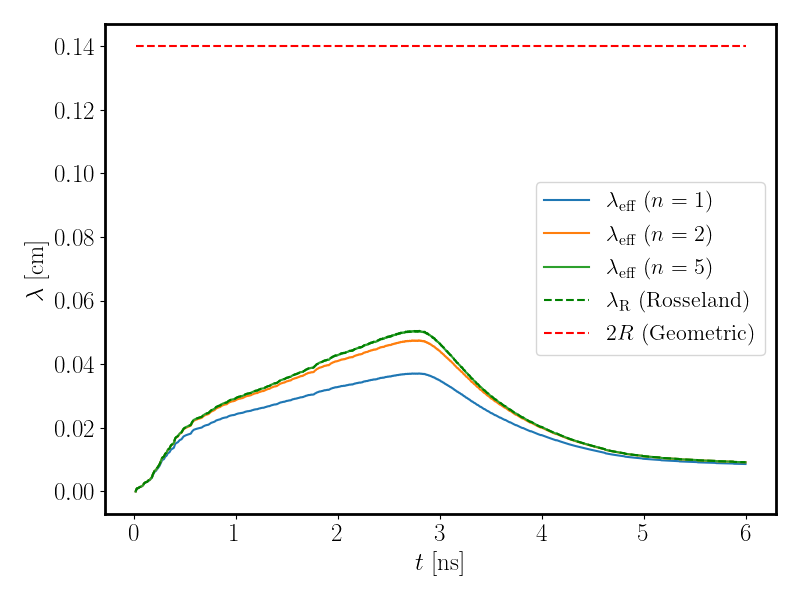
\includegraphics[width=0.45\textwidth]{figures_French22/lambda_eff_vs_time_39.4.png}
    \caption{effective mean free path $\lambda_{\mathrm{eff}}$ and optical depth $\tau$ as functions of time - 39.4 mg/cm$^3$.}
    \label{fig:french22_mfp_with_tau_39p4}
\end{figure}

\section{French2024}
This section is based on a comparison with the experimental data from Courtois et al. (2024)\cite{Courtois2024}. This work contains 2 different experiments, both with a with a SiO$_2$, but one is coated with gold and the other with copper. The first experiment with a SiO$_2$ tube coated with gold, has foam density of $29 [\frac{mg}{cm^3}]$ and diameter of $1 [\mathrm{mm}]$. The second experiment with a SiO$_2$ tube coated with copper, one has foam density of $18.9 [\frac{mg}{cm^3}]$ and diameter of $2 [\mathrm{mm}]$. Each of the experiment has only one point of breakout measured, in the gold coated experiment it is 1.2 mm, and in the copper coated one we have 2.0 mm (which are the tubes lengthes). Another very intresnting data that was measured is the time arrivel of the heatwave front to the end of the tube as a function of the radial location, for both experiments. Both experiments have mfp which is comparable to the tube diameter, and so, an effective MFP correction will be needed here. The gold coated experiment needs a strong correction while the copper coated experiment needs a weaker correction, this can be seen in Fig.~\ref{fig:french24_mfp_with_tau_gold} where we plot the effective mean free path $\lambda_{\mathrm{eff}}$ and optical depth $\tau$ as functions of time for both experiments. The gold coated experiment has a very small optical depth, while the copper coated experiment has a larger optical depth. This is due to the fact that the gold coated experiment has a much smaller tube diameter than the copper coated experiment. The effective mean free path $\lambda_{\mathrm{eff}}$ is calculated using the formula:
\begin{equation}
    \tau(t) = \int_0^{0.9 x_F(t)} \kappa_R(x,t)\rho\,dx, \quad \lambda_R(t) = \frac{0.9\,x_F(t)}{\tau(t)}.
\end{equation}

\begin{figure}[h!]
    \centering
    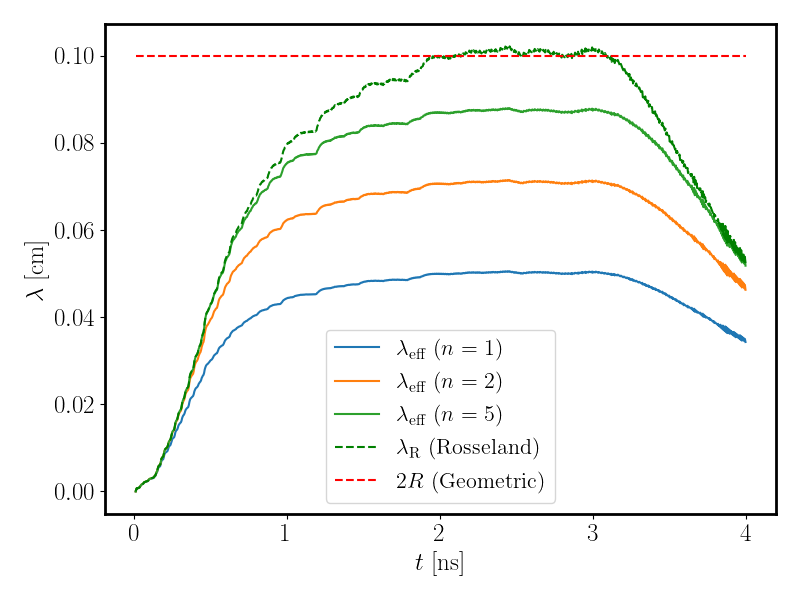
\includegraphics[width=0.48\textwidth]{figures_French24/lambda_eff_vs_time.png}
    \hfill
    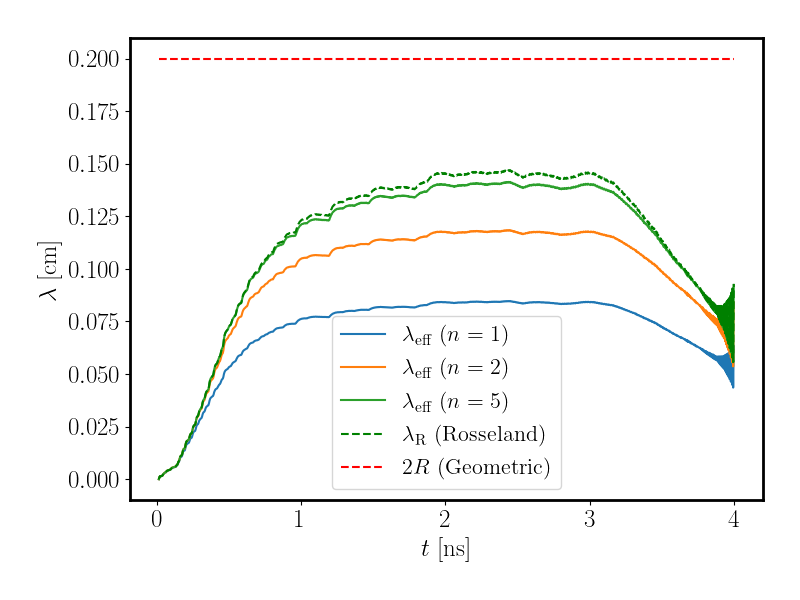
\includegraphics[width=0.5\textwidth]{figures_French24/lambda_eff_vs_time copper.png}
    \caption{Effective mean free path $\lambda_{\mathrm{eff}}$ and optical depth $\tau$ as functions of time for the French2024 cases: gold-coated SiO$_2$ (left) and copper-coated SiO$_2$ (right).}
    \label{fig:french24_mfp_with_tau_gold}
    \label{fig:french24_mfp_with_tau_copper}
\end{figure}

Now for the on-axis propagation of the heatwave front we get Fig.~\ref{fig:french24_front_position_gold} for the gold coated experiment and Fig.~\ref{fig:french24_front_position_copper} for the copper coated experiment. The gold coated experiment is modeled with $n=1$ and FT, while the copper coated experiment is modeled with $n=2.5$ and FT.

\begin{figure}[h!]
    \centering
    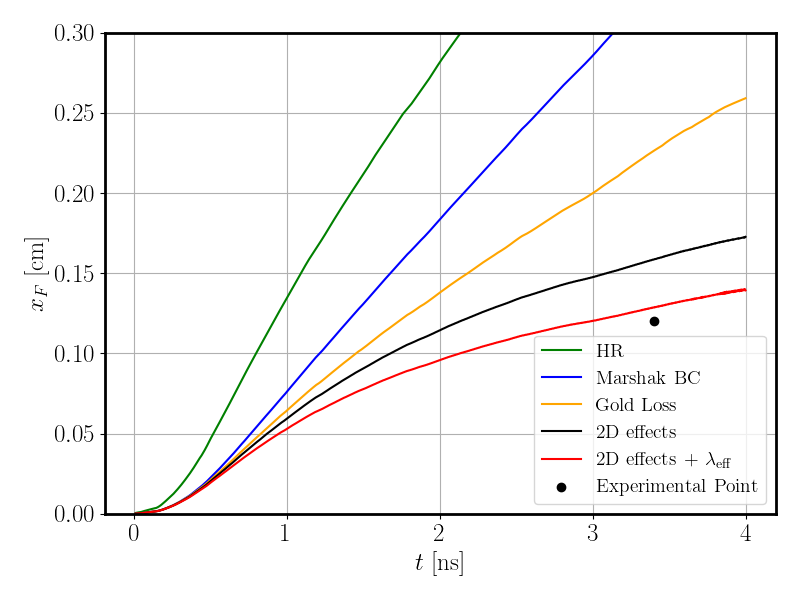
\includegraphics[width=0.6\textwidth]{figures_French24/front_position - french_gold.png}
    \caption{French2024: front position for the SiO$_2$ gold-coating case.}
    \label{fig:french24_front_position_gold}
\end{figure}

\begin{figure}[h!]
    \centering
    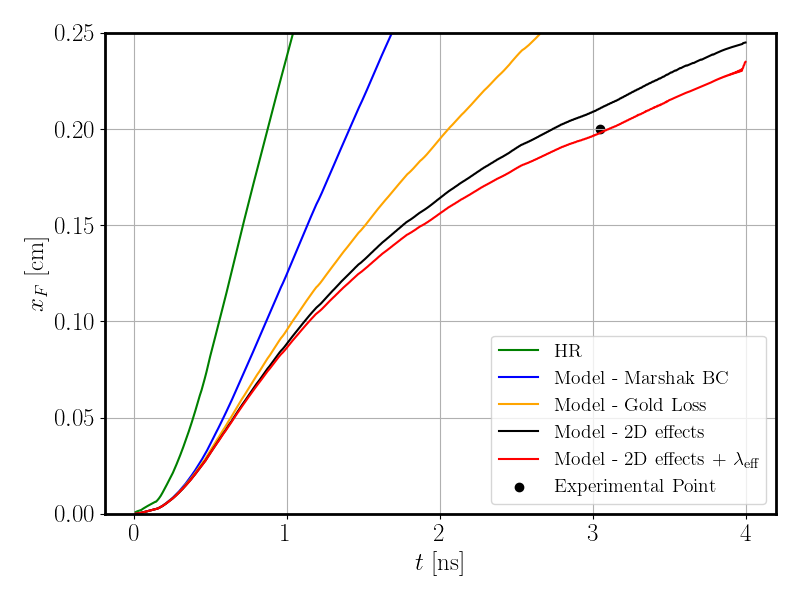
\includegraphics[width=0.6\textwidth]{figures_French24/front_position - french_copper.png}
    \caption{French2024: front position for the SiO$_2$ copper-coating case.}
    \label{fig:french24_front_position_copper}
\end{figure}

Now for the curvature comparison we get Fig.~\ref{fig:french24_curvature} for the curvature of both experiments. The gold coated experiment is modeled with $n=1$ and FT, while the copper coated experiment is modeled with $n=3$ and FT. Note that we used a constant offset to match the initial breakout time of the on-axis heatwave front to the end of the tube, which is $t_{\mathrm{delay}}=0.47\,\mathrm{ns}$ for the gold coated experiment and $t_{\mathrm{delay}}=0.165\,\mathrm{ns}$ for the copper coated experiment. This offset is subtracted from the experimental data arrivel time to match the model predictions.

\begin{figure}[h!]
    \centering
    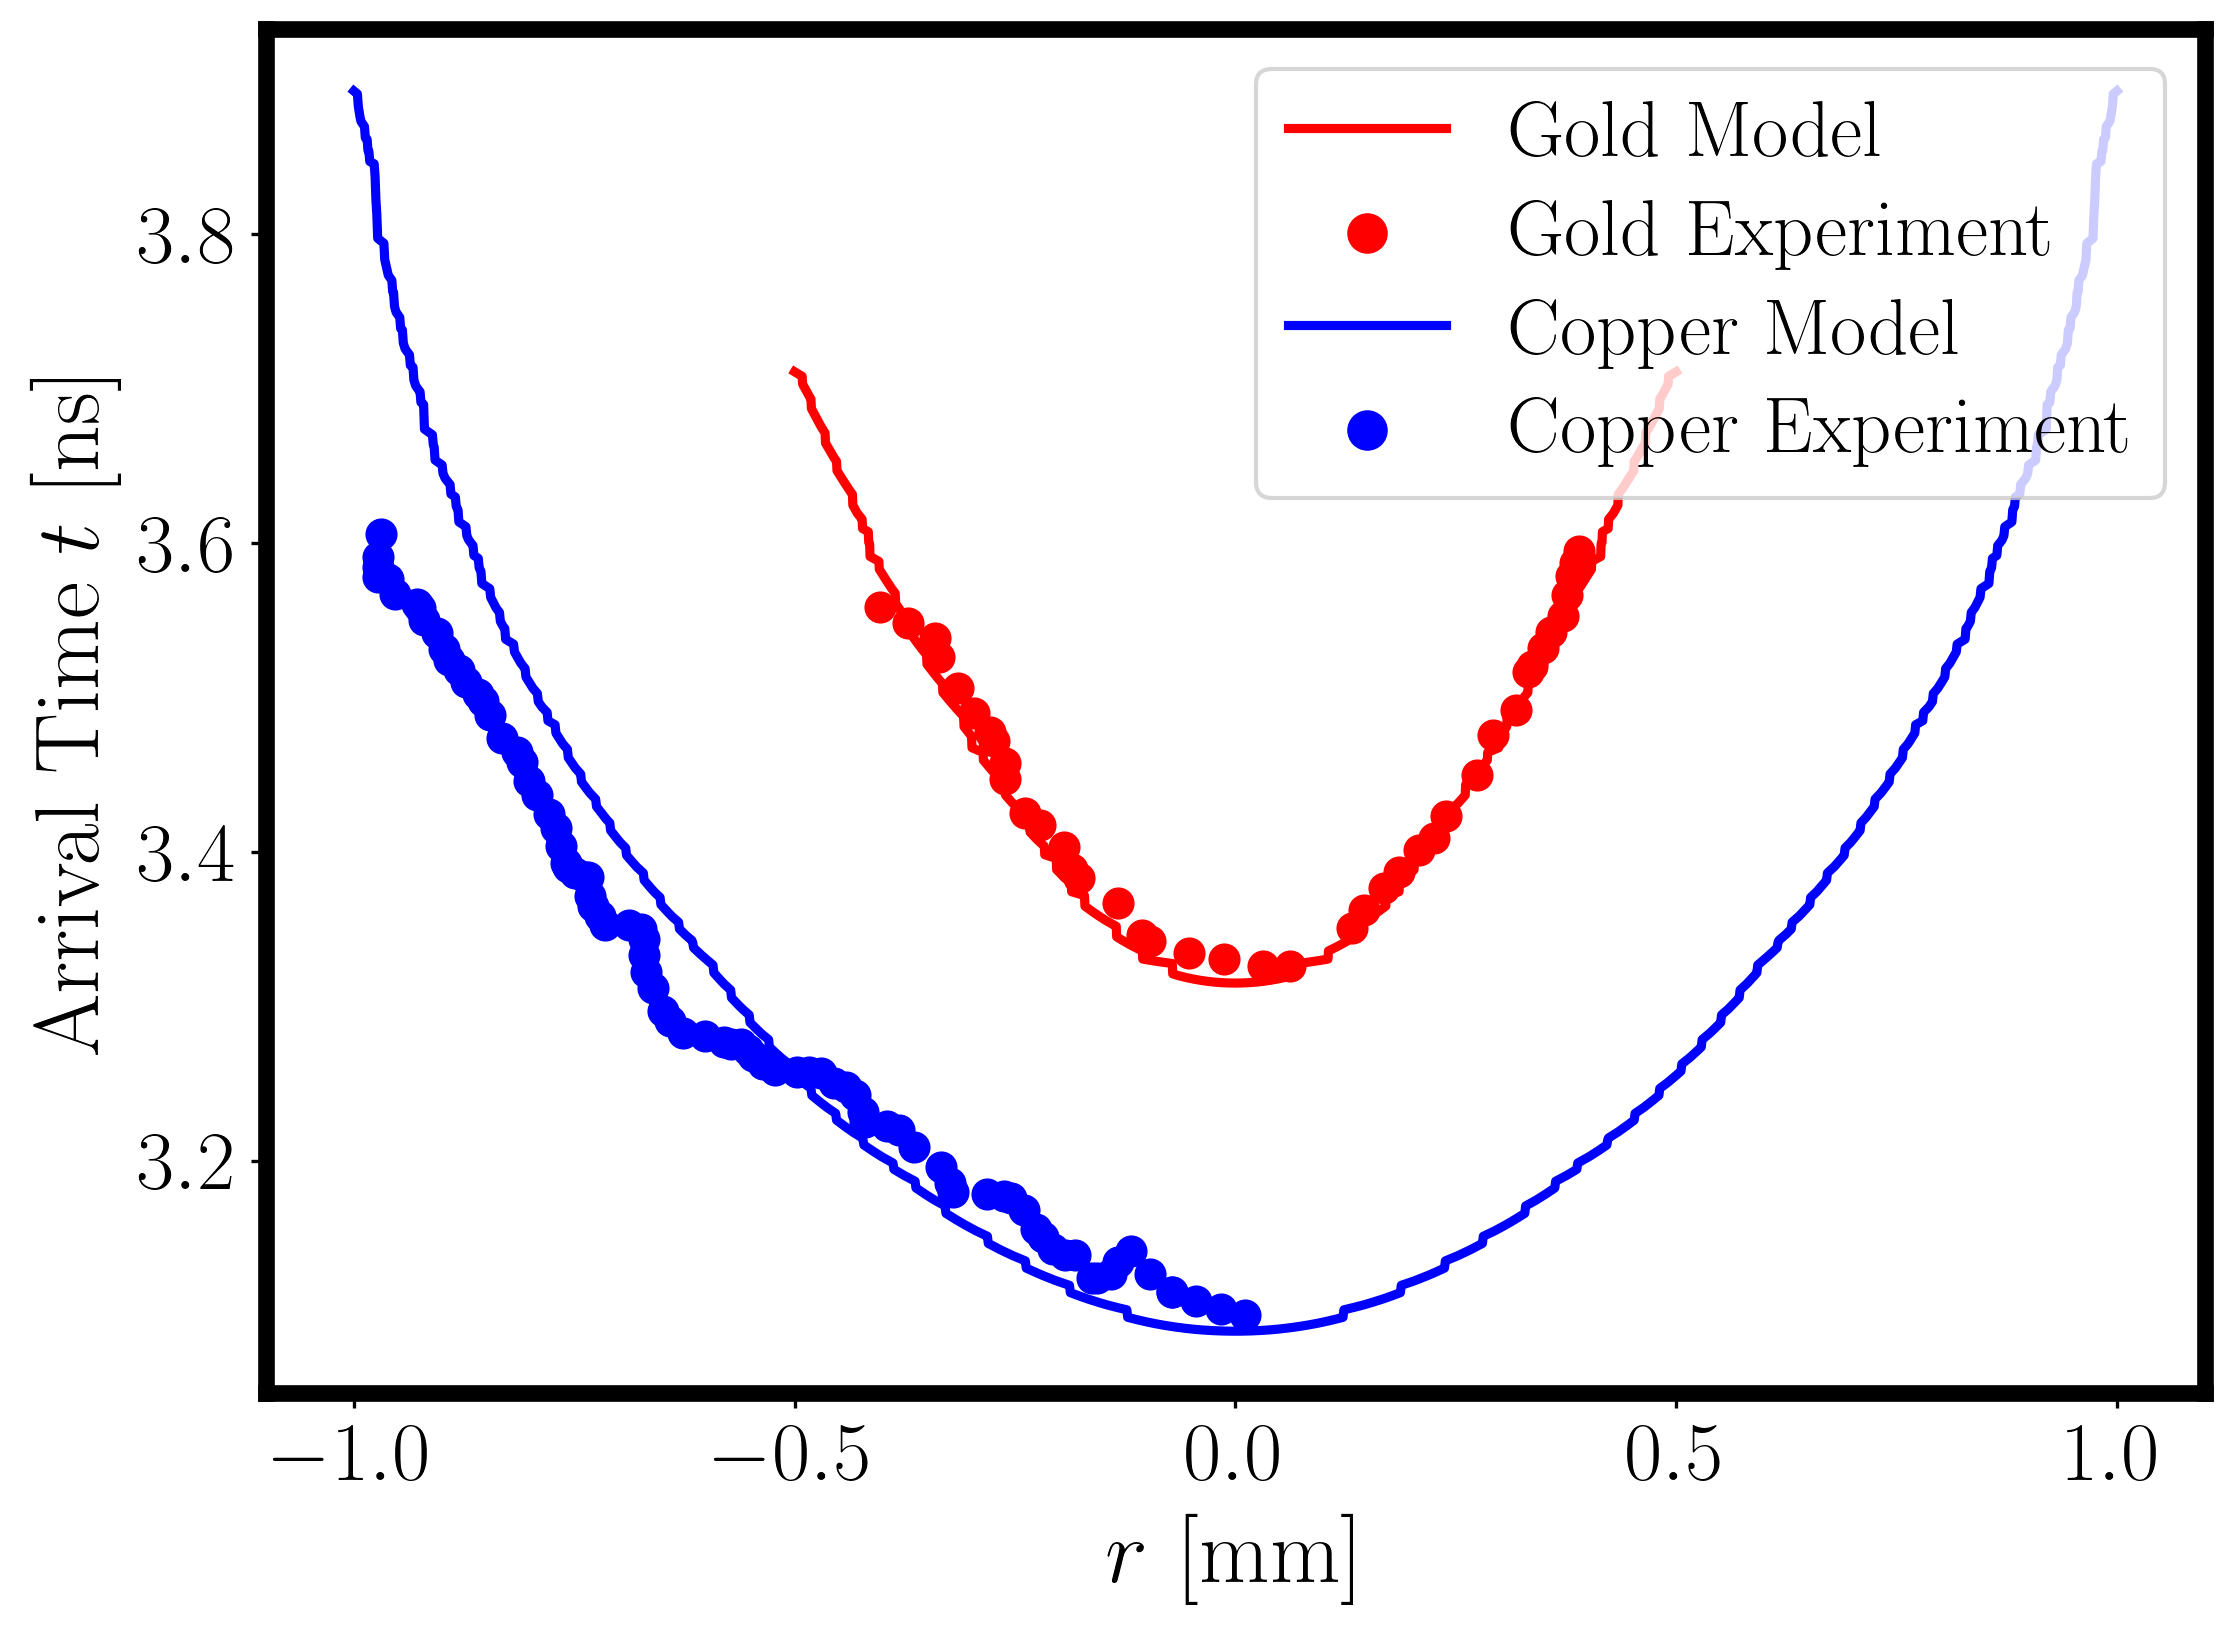
\includegraphics[width=0.5\textwidth]{figures_French24/combined_curvature_comparison.png}
    \caption{French2024: curvature comparison for the SiO$_2$ gold-coating and copper-coating cases}
    \label{fig:french24_curvature}
\end{figure}

\section{Back PRL}
Here we have SiO2 in a 3 mm diamater tubes with 10 mg/cm$^3$ density, and the tubes are coated with gold. We have 4 different tube lengthes: 0.5, 1, 1.5, 2 mm long. The breakout time of the flux is taken as the heat wave time of arrivel to the detector:
\vspace{3em}

\begin{figure}[h]
    \centering
    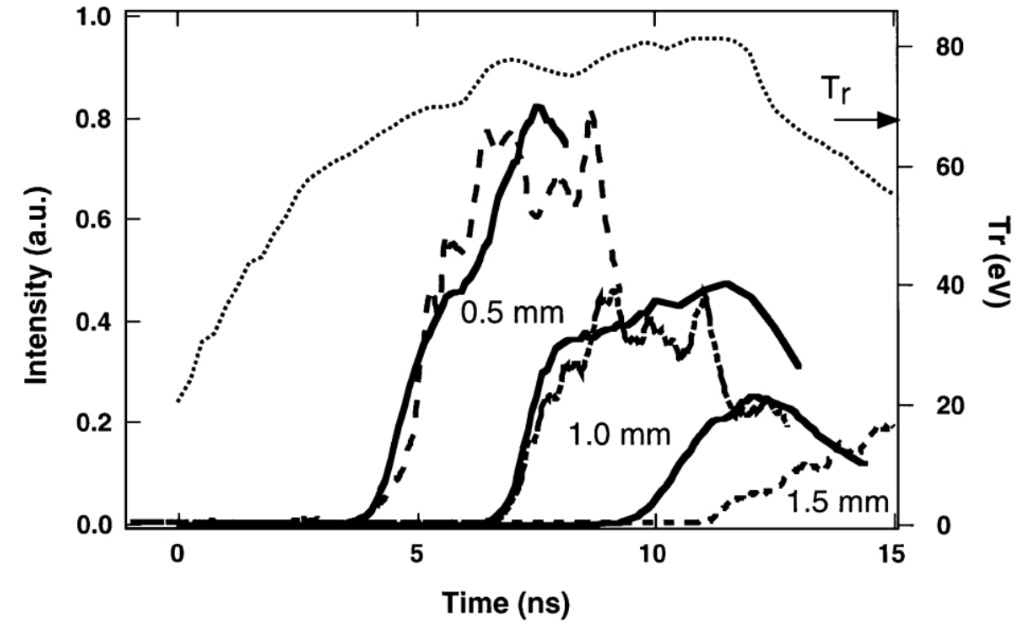
\includegraphics[width=0.5\textwidth]{figures_backPRL/article fluxes.png}
    \caption{Back PRL: fluxes from article for the SiO$_2$ gold-coating case with 3 different tube lengthes.}
    \label{fig:backprl_fluxes}
\end{figure}

Now this experiment is big geometry wise, and so the MFP is much smaller than the tube diameter, and therefore the diffusion approximation is valid, and no mfp correction is needed. We can see that in Fig \ref{fig:backprl_front} even n=1 make almost no change from case with all effects without mfp correction.

\begin{figure}[h]
    \centering
    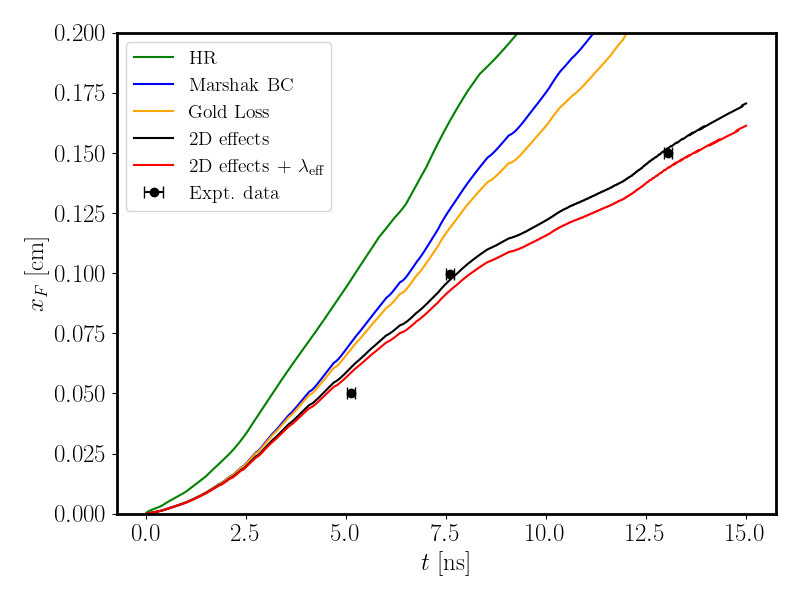
\includegraphics[width=0.475\textwidth]{figures_backPRL/front.png}
    \hfill
    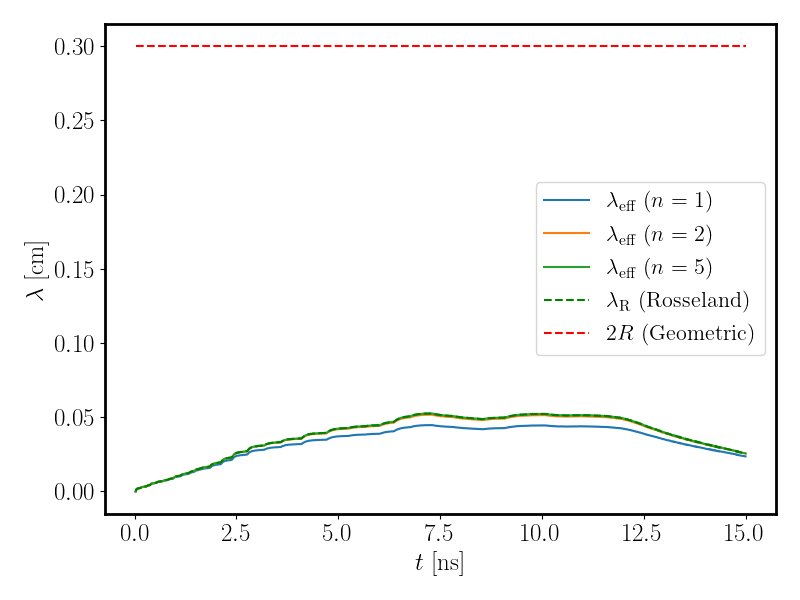
\includegraphics[width=0.47\textwidth]{figures_backPRL/lambda_eff_vs_time.png}
    \caption{Back PRL: front position for the SiO$_2$ gold-coating case with data points 3 different tube lengthes (left), and effective mean free path $\lambda_{\mathrm{eff}}$ as a function of time (right).}
    \label{fig:backprl_front}
\end{figure}

Now the PRL provides us curvature data for 9.5 ns after the drive starts, with tube length of 1mm. Now when comparing with the all the effects, we get Fig.~\ref{fig:backprl_curvature} for the curvature comparison. The model is without mfp correction and FT.

\begin{figure}[h]
    \centering
    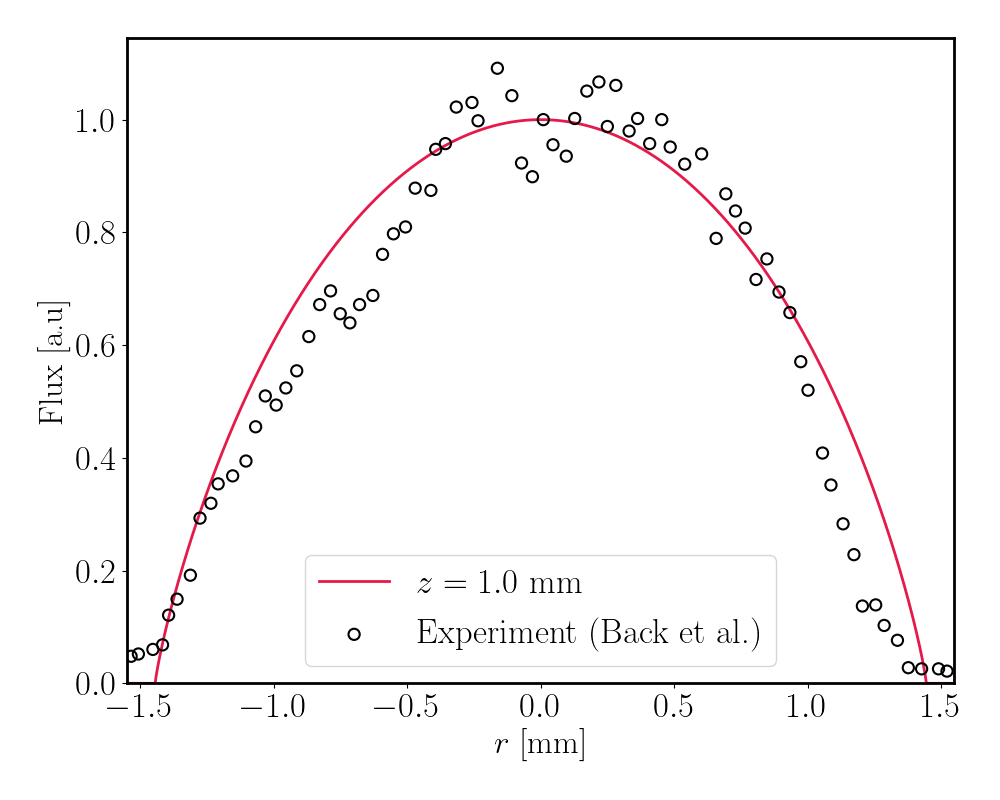
\includegraphics[width=0.5\textwidth]{figures_backPRL/curvature.png}
    \caption{Back PRL: curvature comparison for the SiO$_2$ gold-coating case with tube length of 1 mm.}
    \label{fig:backprl_curvature}
\end{figure}

\vspace{1cm}
\section{Back POP}
\subsection{SiO$_2$}
For the SiO$_2$ experiment reported by Back \textit{et al.}~\cite{Back2000POP}, the model uses the \texttt{SiO2} parameters: an initial foam density of $0.05\,\mathrm{g\,cm^{-3}}$ ($50\,\mathrm{mg\,cm^{-3}}$) and a tube radius of $0.16\,\mathrm{cm}$ (diameter $1.6\,\mathrm{mm}$). The gold-wall comparison in Fig.~\ref{fig:backpop_front} includes three measured heat-front breakout times, defined by the moment when the flux reaches half its maximum value. This criterion does not mark the very first arrival of the heat front; as discussed for the earlier experiment, however, using this half-maximum definition has a negligible effect on the inferred front trajectory. The comparison also illustrates the importance of energy loss to the gold wall: among the modeled effects, wall loss produces the largest slowing of the front. The red curve includes the combined effects, including the effective-mean-free-path correction with limiter power $n=1.2$, and uses a flat-top (FT) approximation. This choice gives the best agreement with the measured front positions.

The right panel of Fig.~\ref{fig:backpop_front} shows $\lambda_{\mathrm{eff}}$ for several limiter exponents. Its peak values are a substantial fraction of the tube diameter, $0.16\,\mathrm{cm}$, indicating that the finite-mean-free-path correction is not negligible for this geometry. Including this correction further improves the agreement between the modeled and measured front positions.

\begin{figure}[h]
    \centering
    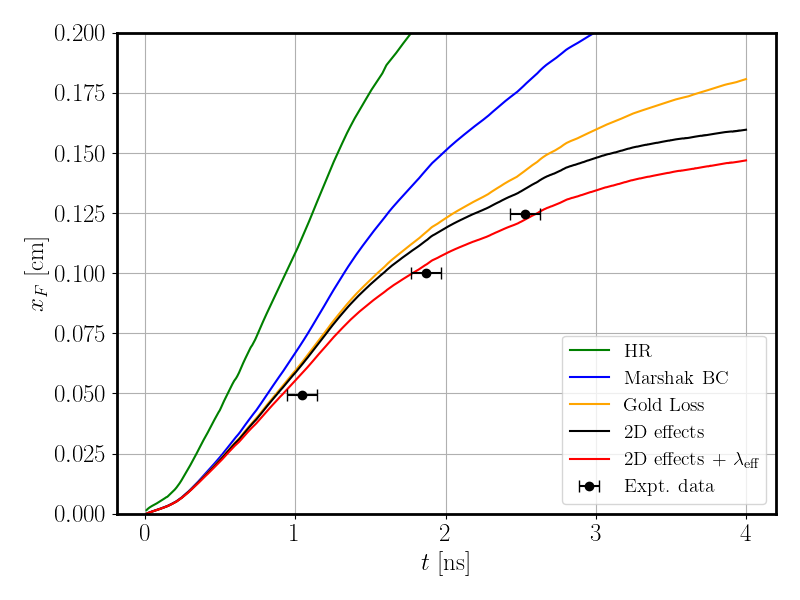
\includegraphics[width=0.475\textwidth]{figures_backPOP/front.png}
    \hfill
    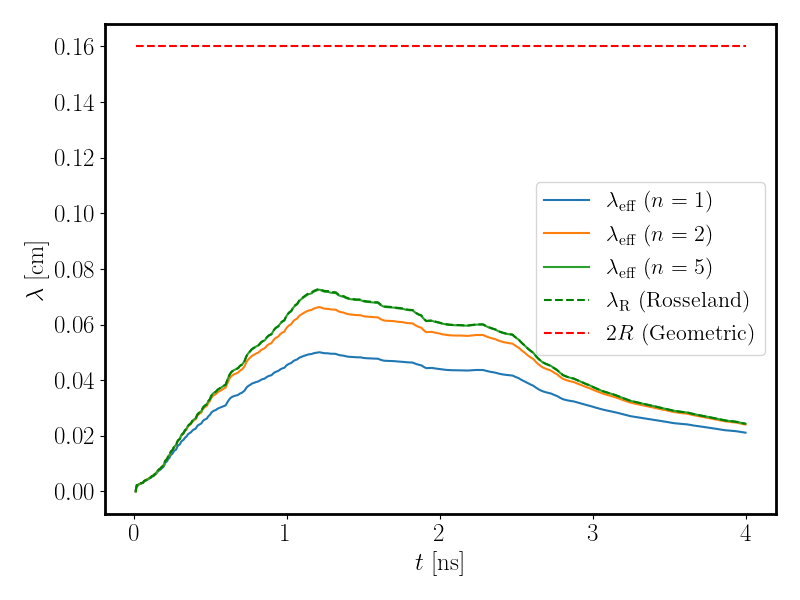
\includegraphics[width=0.47\textwidth]{figures_backPOP/lambda_eff_vs_time.png}
    \caption{Back POP: front position for the SiO$_2$ gold-coating case with data points 3 different tube lengthes (left), and effective mean free path $\lambda_{\mathrm{eff}}$ as a function of time (right).}
    \label{fig:backpop_front}
\end{figure}

Having accounted for the corrections to the longitudinal front propagation, we next assess the full two-dimensional heat-front shape against the numerical simulation, as shown in Fig.~\ref{fig:backpop_front_curvature}. This comparison must be interpreted within the limitations of the simulation, which does not include hydrodynamics. Accordingly, the model uses the supersonic wall-heating formulas for both gold and copper, rather than a hydrodynamic ablation treatment. Unlike the preceding comparison with the experimental breakout times, the flat-top approximation does not adequately reproduce the simulated radial front shape; we therefore use the Henyey profile (\texttt{FT=False}). The effective-mean-free-path limiter exponents are $n=2$ for Be, $n=0.9$ for vacuum, $n=1.3$ for copper, and $n=2$ for gold. At $t=2.5\,\mathrm{ns}$, the model reproduces both the coating-dependent ordering of the front positions and the change in radial curvature: the gold and copper cases have relatively flat fronts, whereas the Be and vacuum cases show stronger bending near the tube wall. Agreement is generally good across the radial domain, although some differences remain near the wall, particularly for Be and copper. For gold, the comparison at $t=1$, $2$, and $2.5\,\mathrm{ns}$ also shows good agreement in both front position and shape, indicating that the agreement is maintained over time rather than being restricted to a single snapshot.

\begin{figure}[h]
    \centering
    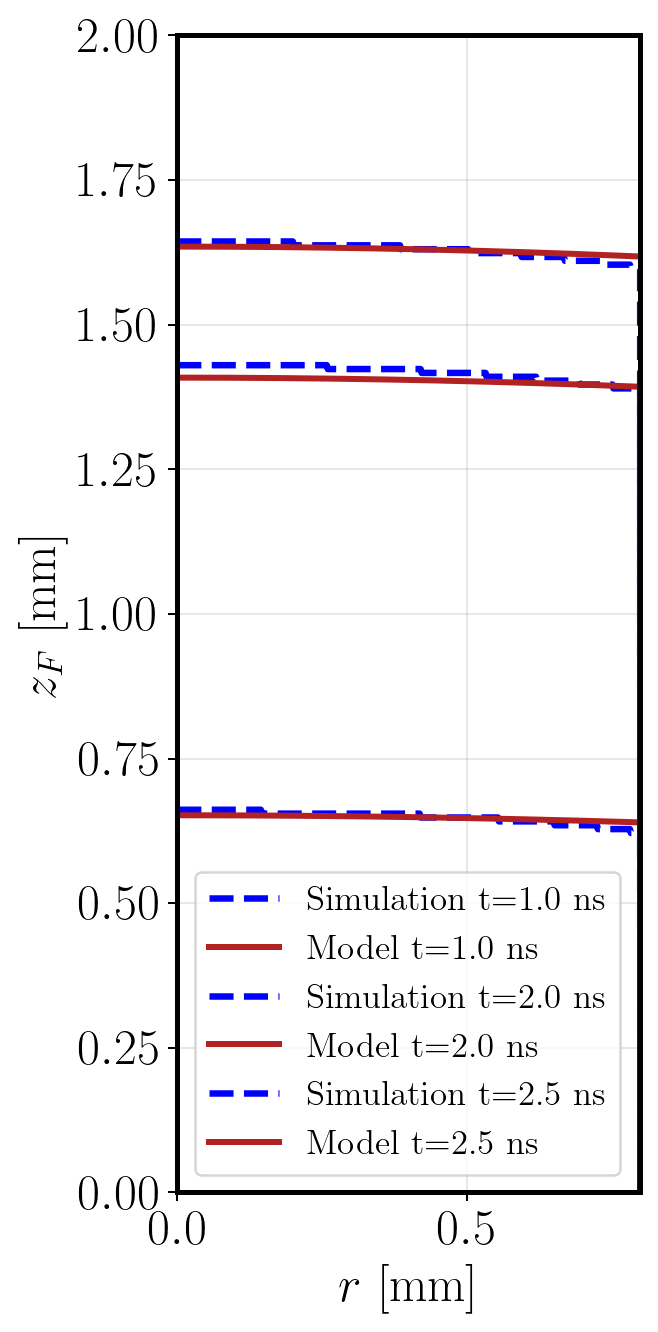
\includegraphics[width=0.24\textwidth]{figures_backPOP/front_surface.png}
    \hfill
    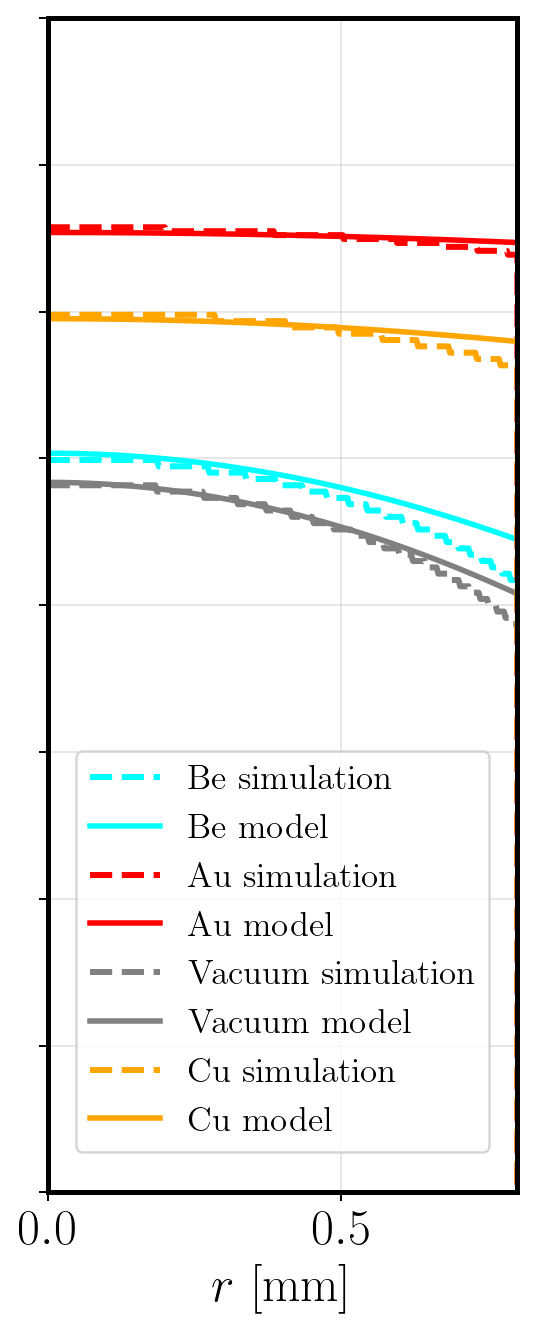
\includegraphics[width=0.195\textwidth]{figures_backPOP/all_coatings_front_surface_t2.5ns.png}
    \caption{Two-dimensional heat-front shapes for the Back POP SiO$_2$ case: model--simulation comparison for gold at $t=1$, $2$, and $2.5\,\mathrm{ns}$ (left), and comparison of Be, gold, vacuum, and copper cases at $t=2.5\,\mathrm{ns}$ (right). Dashed curves denote the simulation and solid curves the model. The model uses the Henyey profile, with effective-mean-free-path limiter exponents $n=2$ (Be), $0.9$ (vacuum), $1.3$ (copper), and $2$ (gold).}
    \label{fig:backpop_front_curvature}
\end{figure}


\subsection{Ta$_2$O$_5$}
The model uses the parameters specified for \texttt{Ta2O5}: an initial density of $0.04\,\mathrm{g\,cm^{-3}}$ ($40\,\mathrm{mg\,cm^{-3}}$) and a tube diameter of $D=0.16\,\mathrm{cm}$. Figure~\ref{fig:backpop_front_ta2o5} shows two distinct experiments (using the same foam - the Ta$_2$O$_5$ foam): the gold-coated targets reported in the Physics of Plasmas article by Back \textit{et al.}~\cite{Back2000POP}, and the Be-coated targets described in the annual report by Landen \textit{et al.}~\cite{Landen2000}. The last tested the effect of an optically thin beryllium instead of an optically thick gold sleeve. Although a full account of the Be experiment has not been published, the available report gives breakout times for $0.5$ and $1\,\mathrm{mm}$ foam lengths that are approximately $10\%$ later than those measured with gold.

The distinction between the wall-heating regimes is important for interpreting this comparison. Throughout the temperature range considered here, the heat wave in Be is supersonic rather than subsonic; the Be wall is therefore treated using the supersonic formulas, without hydrodynamics. In contrast, the gold-wall calculation includes ablation, which further slows the foam heat front. With gold-wall ablation included, the Be-coated case propagates only slightly more slowly than the gold-coated case, not completely consistent with the modest separation between the measured breakout times. The cyan curve represents the supersonic Be-wall calculation, while the red curve includes gold-wall ablation. Both use the flat-top (FT) approximation and the effective-mean-free-path correction with limiter exponent $n=1$. I thing that the main reason that the beryllium case does not perfectly match the modest separation in breakout times is the missing accuracy in the wall curvature when using the flattop assumption on Be (since we lose a lot of the energy near the wall).

The right panel shows that $\lambda_{\mathrm{eff}}$ is small compared to the tube radius, indicating that the finite-mean-free-path correction is relatively minor for the Ta$_2$O$_5$ conditions considered here.

\begin{figure}[h]
    \centering
    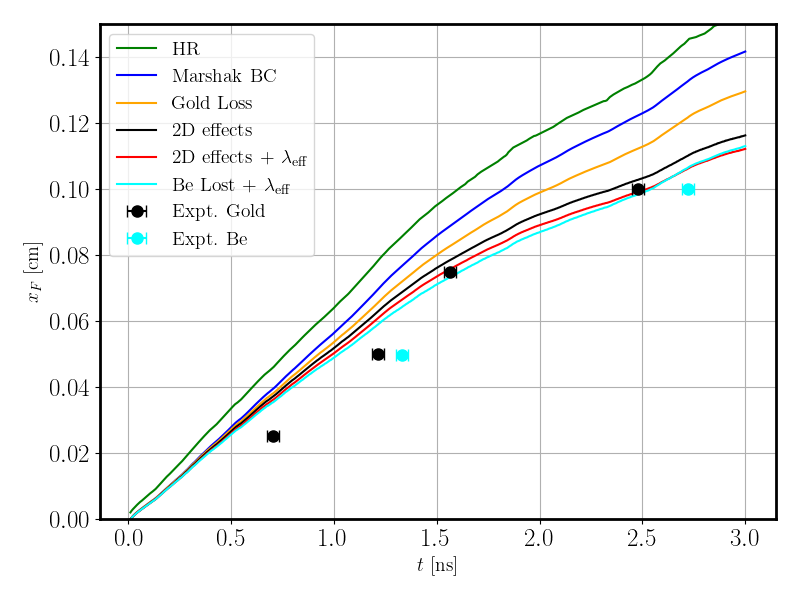
\includegraphics[width=0.475\textwidth]{figures_backPOP/front2.png}
    \hfill
    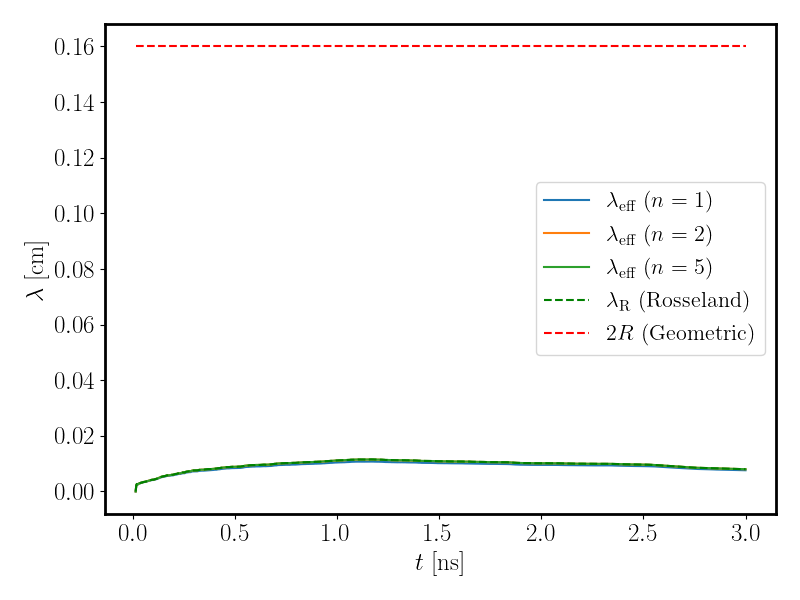
\includegraphics[width=0.47\textwidth]{figures_backPOP/lambda_eff_vs_time2.png}
    \caption{Ta$_2$O$_5$ comparison: front propagation for the gold-coated experiment reported in Physics of Plasmas~\cite{Back2000POP} and the Be-coated experiment described in the annual report~\cite{Landen2000} (left), and effective mean free path $\lambda_{\mathrm{eff}}$ as a function of time (right). The cyan and red model curves use the FT approximation and limiter exponent $n=1$, with supersonic wall heating for Be and wall ablation for gold, respectively.}
    \label{fig:backpop_front_ta2o5}
\end{figure}

We next examine the radial flux profiles of the gold-coated Ta$_2$O$_5$ targets shown in Fig.~9 of Back \textit{et al.}~\cite{Back2000POP}. These profiles were measured $500\,\mathrm{ps}$ ($0.5\,\mathrm{ns}$) after breakout for foam lengths of $0.25$, $0.5$, $0.75$, and $1.0\,\mathrm{mm}$. To construct the corresponding model profiles, we extract radial cross sections of the temperature map at each axial position and evaluate the flux at a delay of $0.5\,\mathrm{ns}$ relative to the local front-arrival time. As shown in Fig.~\ref{fig:backpop_front_ta2o5}, however, the model predicts breakout approximately $0.1\,\mathrm{ns}$ earlier than the experiment for the $0.25$ and $0.5\,\mathrm{mm}$ targets. We therefore shift the model breakout times for these two targets by $+0.1\,\mathrm{ns}$ before applying the $0.5\,\mathrm{ns}$ sampling delay, aligning the comparison with the experimental timing. No timing correction is applied to the two longer targets. The model and experimental profiles are normalized separately to the on-axis flux of their respective $0.25\,\mathrm{mm}$ target profiles. As shown in Fig.~\ref{fig:backpop_flux_curvature_post_breakout_ta2o5}, the shorter-target profiles are reproduced more closely, whereas the longer-target measurements are flatter and extend farther radially than the model predictions.

The broader, flatter profiles measured for the $0.75$ and $1.0\,\mathrm{mm}$ Ta$_2$O$_5$ targets reveal a limitation of the present model. Our model is restricted to the diffusion approximation and estimates the emerging flux from the local temperature through $F\propto T^4$, rather than explicitly calculating radiation transport to the detector. Although this approximation is useful in optically thick conditions, it cannot capture nonlocal contributions to the detected intensity when photons escape from a range of depths or propagate through relatively transparent spectral bands. Such transport effects could contribute to the discrepancy for the two longer targets. However, the measured profile shapes alone do not establish a transition to a transport-dominated regime or explain why the discrepancy increases with length; resolving this requires frequency-dependent optical depths and a transport calculation incorporating the detector response.

\begin{figure}[h]
    \centering
    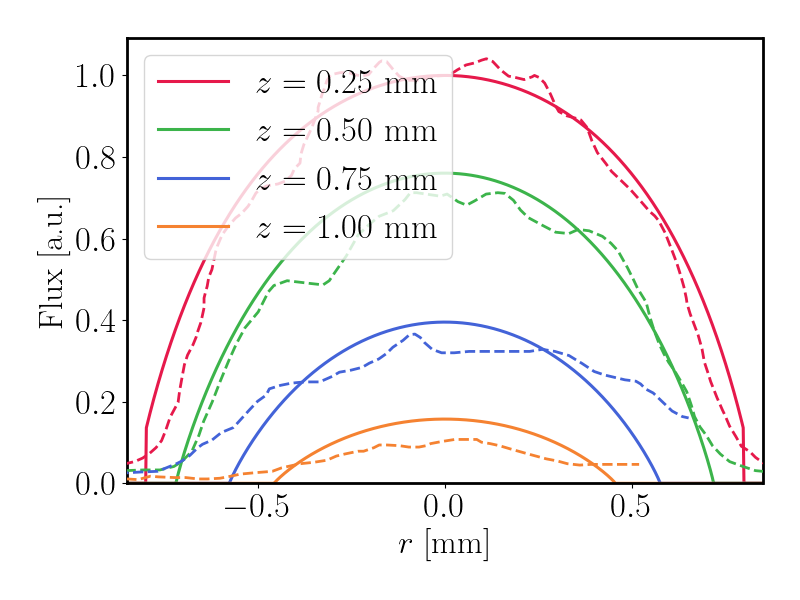
\includegraphics[width=0.5\textwidth]{figures_backPOP/flux_curvature_post_breakout_0.5ns.png}
    \caption{Ta$_2$O$_5$ comparison: flux curvature post breakout at $0.5\,\mathrm{ns}$ delay for the gold-coated experiment~\cite{Back2000POP} . The cyan and red model curves use the FT approximation and limiter exponent $n=1$, with supersonic wall heating for Be and wall ablation for gold, respectively.}
    \label{fig:backpop_flux_curvature_post_breakout_ta2o5}
\end{figure}

The annual report~\cite{Landen2000} also allows a comparison of the radial emission profiles from Be- and gold-coated Ta$_2$O$_5$ targets. Figure~18 on page~120 presents radial emissivity measurements taken $200\,\mathrm{ps}$ after radiation breakout from $0.5\,\mathrm{mm}$-long foams with an initial density of $40\,\mathrm{mg\,cm^{-3}}$. The semi-analytic model does not reproduce the measured Be profile well, suggesting a limitation in its treatment of the coupled effects shaping the radial emission, even though these effects can be treated individually. Since wall heating in Be remains supersonic over the temperature range considered here, we can also compare the measurements with a two-dimensional radiation-diffusion simulation without hydrodynamics. We extract the simulated radial flux profile at $z=0.5\,\mathrm{mm}$, $200\,\mathrm{ps}$ after the simulated front reaches that position. Although the simulation domain extends beyond the experimental target length, this internal cross section gives substantially better agreement with the measured Be profile; it is not, however, a direct calculation of emission from a finite target's exit surface. For the semi-analytic comparison, the sampling time is taken as $t_{\mathrm{sample}}=t_{\mathrm{breakout,model}}+0.2\,\mathrm{ns}+0.1\,\mathrm{ns}$, where the additional $0.1\,\mathrm{ns}$ is an empirical timing adjustment. The flat-top approximation does not adequately reproduce the profile in this case, so we instead use the Henyey profile (\texttt{FT=False}). We also didnwt use the effective MFP effect.

\begin{figure}[h]
    \centering
    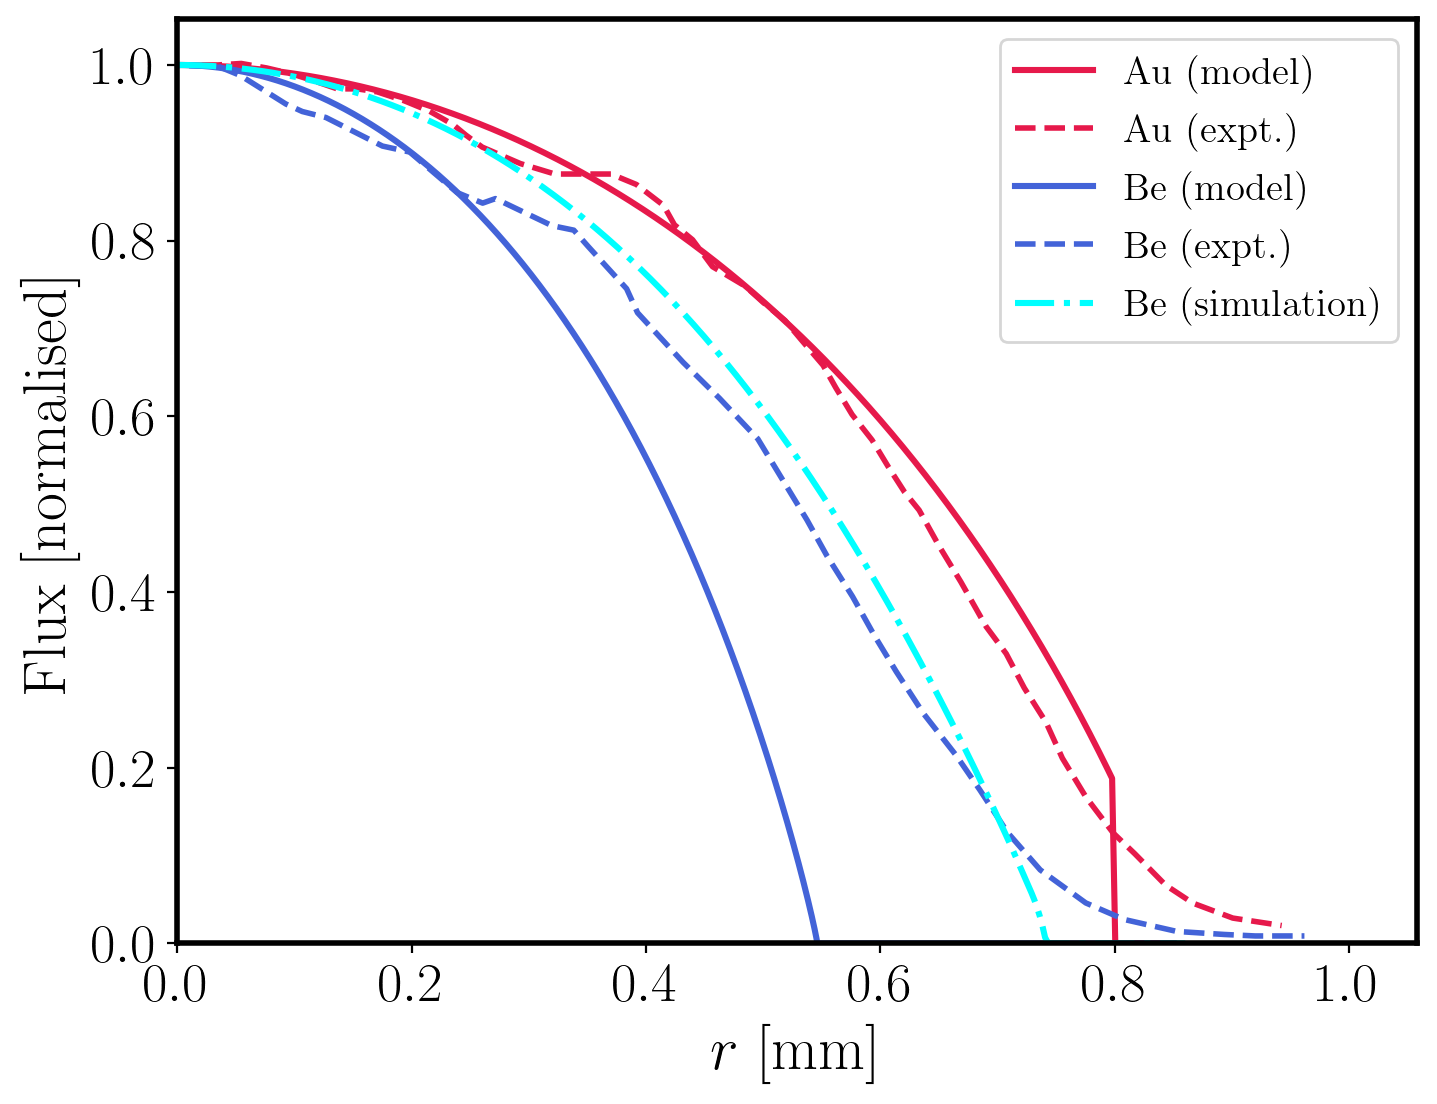
\includegraphics[width=0.34\textwidth]{figures_backPOP/flux_curvature_be_vs_gold.png}
    \hfill
    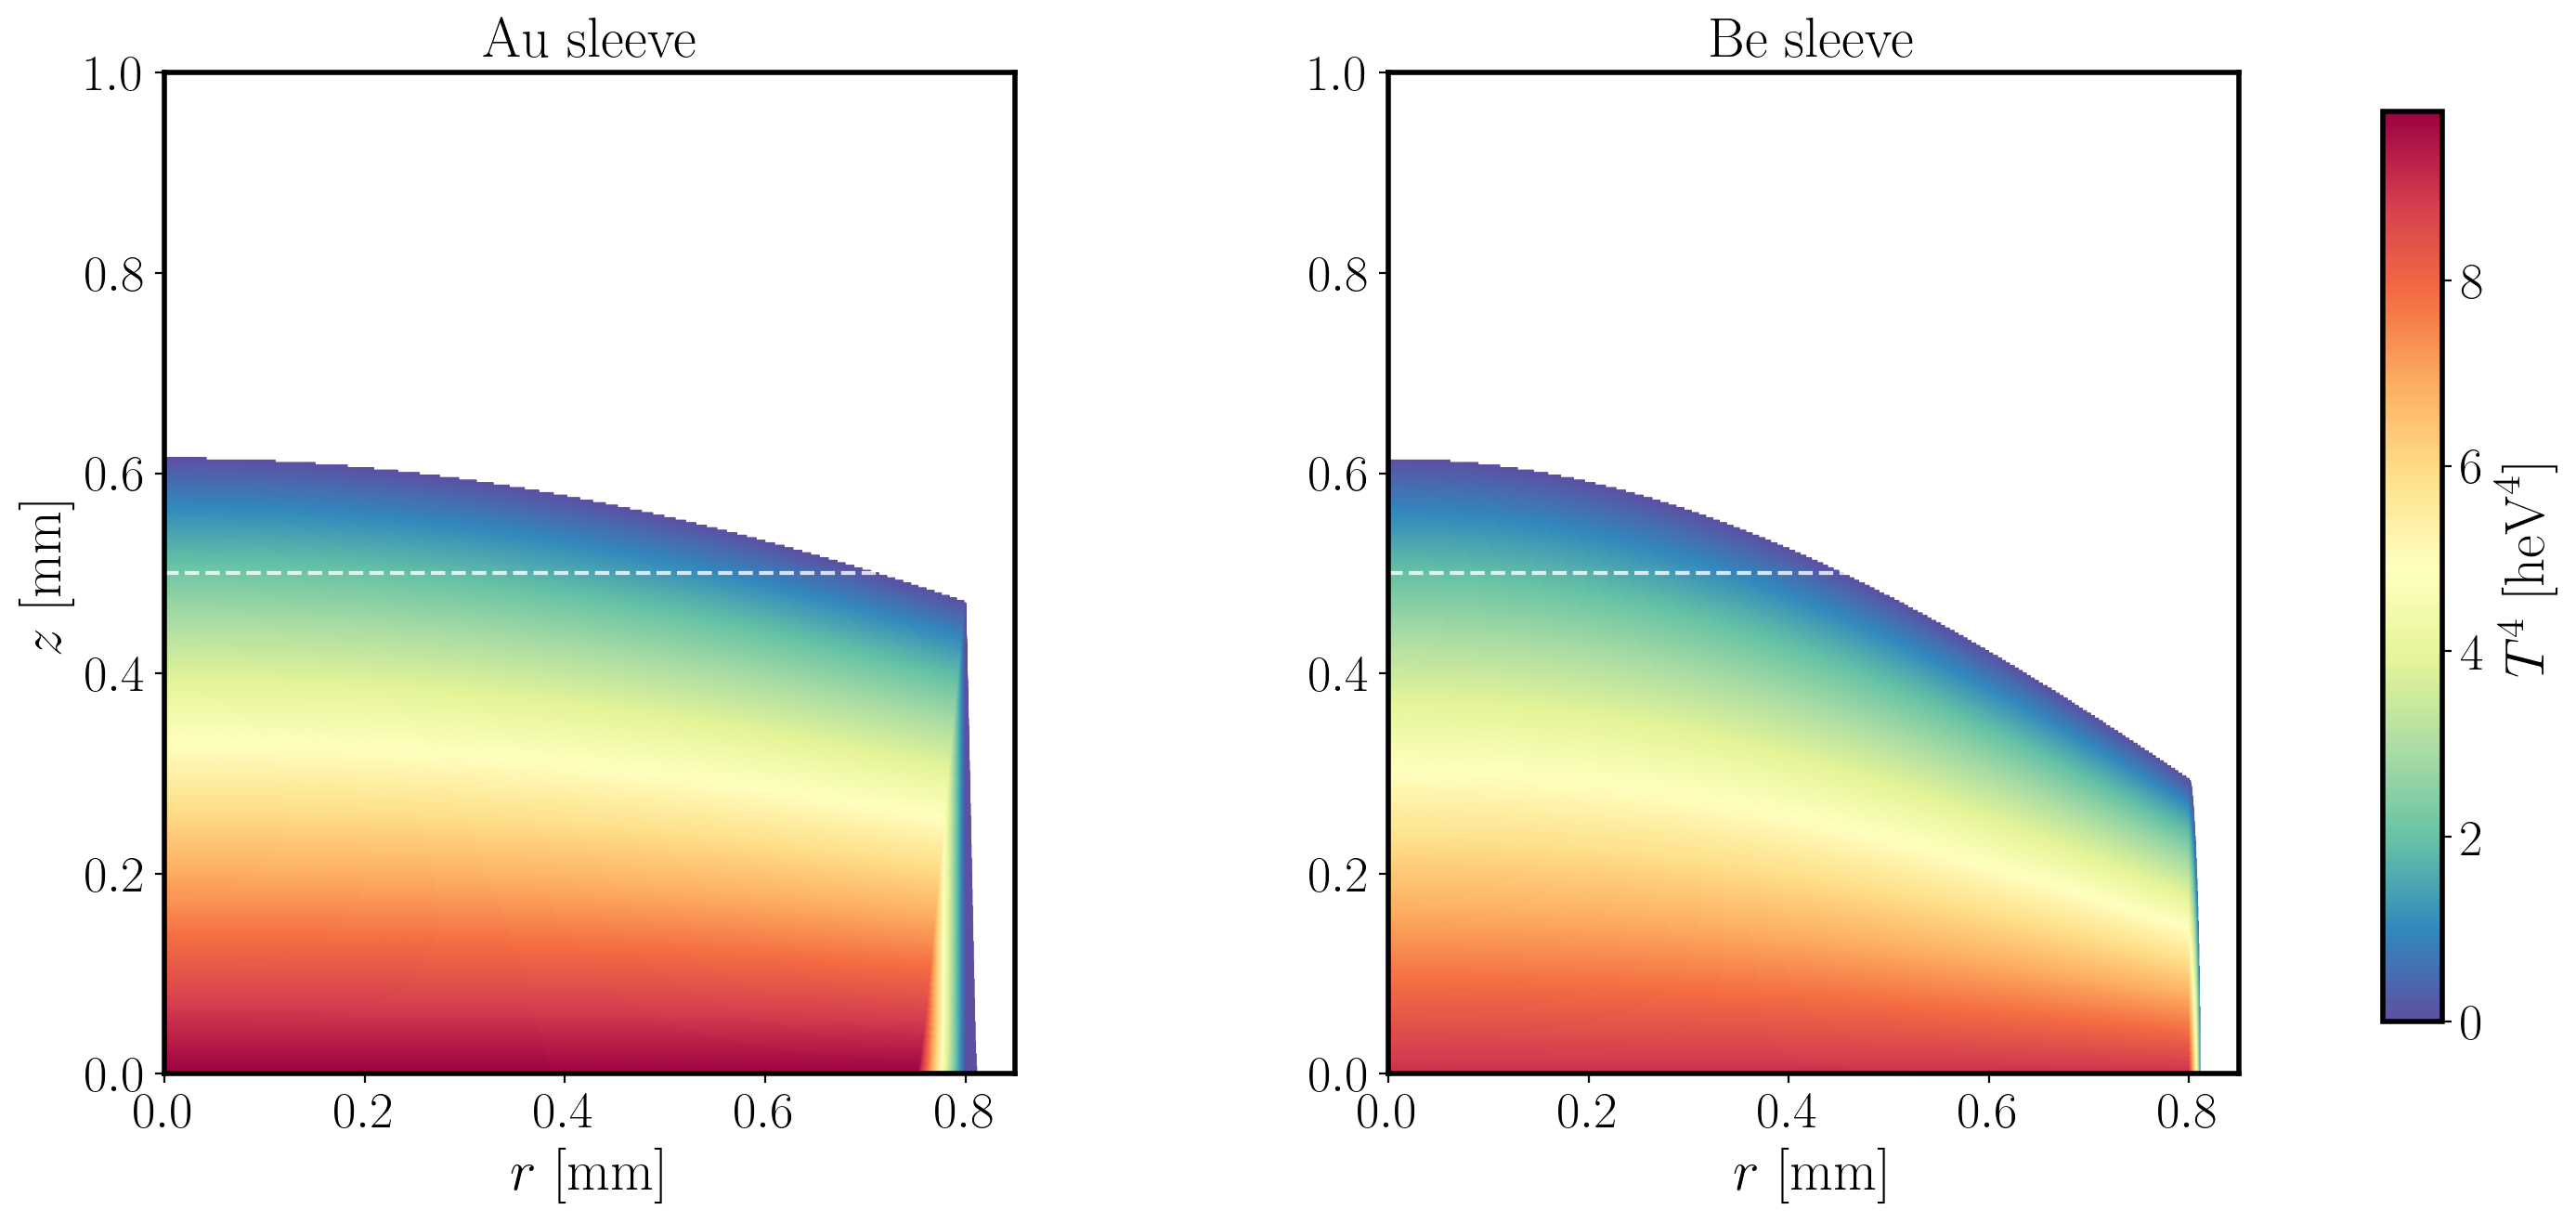
\includegraphics[width=0.57\textwidth]{figures_backPOP/T4_heatmap_be_vs_gold.png}
    \caption{Comparison of flux curvature (left) and $T^4$ heatmap (right) for Be- and gold-coated Ta$_2$O$_5$ targets.}
    \label{fig:backpop_front_ta2o5}
\end{figure}

\vspace{1em}

Returning to the Physics of Plasmas measurements~\cite{Back2000POP}, we compare the radial emission profiles of $1\,\mathrm{mm}$-long SiO$_2$ and Ta$_2$O$_5$ targets, measured $400\,\mathrm{ps}$ after on-axis breakout. Figure~\ref{fig:backpop_flux_curvature_sio2_vs_ta2o5} shows a substantially narrower, more centrally peaked profile for Ta$_2$O$_5$, whereas the SiO$_2$ emission is flatter across the tube. This difference is consistent with the lower optical thickness of SiO$_2$, which allows radiation to propagate more readily through the foam. The measured longitudinal propagation also differs: the SiO$_2$ front reaches $1\,\mathrm{mm}$ in less than $2\,\mathrm{ns}$, whereas the Ta$_2$O$_5$ front reaches the same position at approximately $2.5\,\mathrm{ns}$. The shorter propagation time in SiO$_2$ leaves less time for cumulative wall losses, which may contribute to its flatter radial profile. However, the front-arrival times alone do not determine the radial energy loss; the emission shape also depends on the temperature distribution, wall coupling, and radiation transport.

Both model profiles use the flat-top (FT) approximation and the effective-mean-free-path correction with limiter exponent $n=1$. For Ta$_2$O$_5$, the profile is sampled $0.4\,\mathrm{ns}$ after the calculated on-axis breakout, matching the nominal experimental delay. For SiO$_2$, a shorter model sampling delay of $0.2\,\mathrm{ns}$ is used to obtain closer agreement with the measured profile; among the delays examined, $0.15\,\mathrm{ns}$ gave the closest visual agreement. This adjustment is empirical and should not be interpreted as a comparison at identical post-breakout times or as an independent validation of the model timing.

\begin{figure}[h]
    \centering
    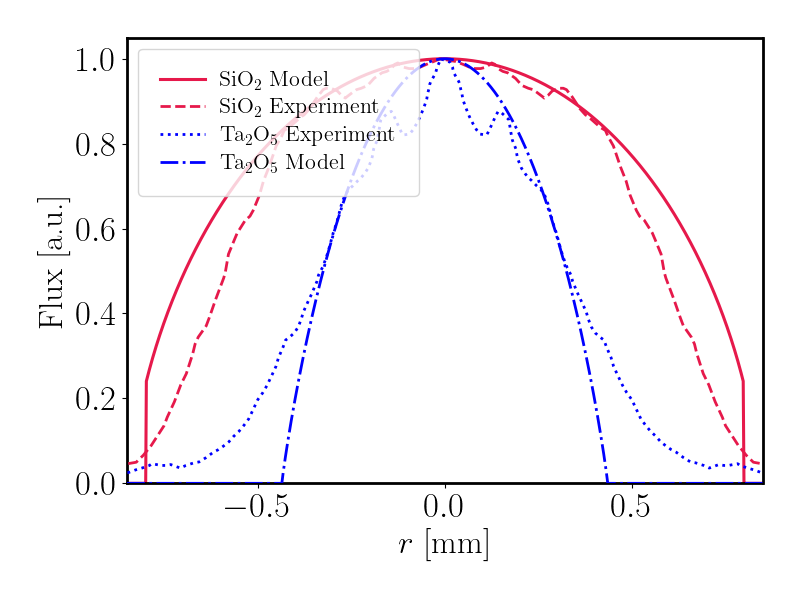
\includegraphics[width=0.45\textwidth]{figures_backPOP/flux_curvature_post_breakout_0.4ns}
    \caption{Radial emission profiles of $1\,\mathrm{mm}$-long SiO$_2$ and Ta$_2$O$_5$ targets. Experimental profiles were measured $0.4\,\mathrm{ns}$ after on-axis breakout~\cite{Back2000POP}; model profiles use sampling delays of $0.2\,\mathrm{ns}$ for SiO$_2$ and $0.4\,\mathrm{ns}$ for Ta$_2$O$_5$. Both calculations use the FT approximation and effective-mean-free-path limiter exponent $n=1$.}
    \label{fig:backpop_flux_curvature_sio2_vs_ta2o5}
\end{figure}

\section{Ji-Yan}
Zhang \textit{et al.}~\cite{Zhang2010} investigated ionization and shock fronts in foam targets driven by thermal radiation. Here we compare the calculated radiation heat-front trajectory with the experimental points used in the Ji-Yan comparison. The model represents the foam as C$_8$H$_8$, with an initial density of $0.16\,\mathrm{g\,cm^{-3}}$ ($160\,\mathrm{mg\,cm^{-3}}$) and radius $R=0.01\,\mathrm{cm}$ (diameter $0.2\,\mathrm{mm}$). The calculation uses a vacuum lateral boundary to account for radiative escape, rather than a surrounding metal sleeve. 

The left panel of Fig.~\ref{fig:jiyan_front_and_mfp} illustrates the successive corrections to the longitudinal propagation. The uncorrected HR solution substantially overpredicts the measured front position. Applying the Marshak boundary condition reduces the predicted propagation speed, and including lateral radiative losses brings the trajectory closer to the measurements. The red curve additionally includes the effective-mean-free-path correction with limiter exponent $n=1$ and gives the closest agreement among the plotted models, although some overprediction remains, particularly at earlier times. In the paper~\cite{Zhang2010}, they note that the breakout time of the experimental front points was measured experimentally at half-maximum peak-emissivity points. However, taking this into account slow the front too much and we get no agreement with the data.

The right panel explains why the finite-mean-free-path correction is important for this narrow target. The geometric restriction on radiation transport is consequently significant, consistent with the improved front-position agreement when the correction is included. Since the Rosseland mean free path is comparable to the target's transverse dimension, however, this correction should be regarded as an effective treatment within the diffusion model, not a replacement for a full transport calculation.

\begin{figure}[h]
    \centering
    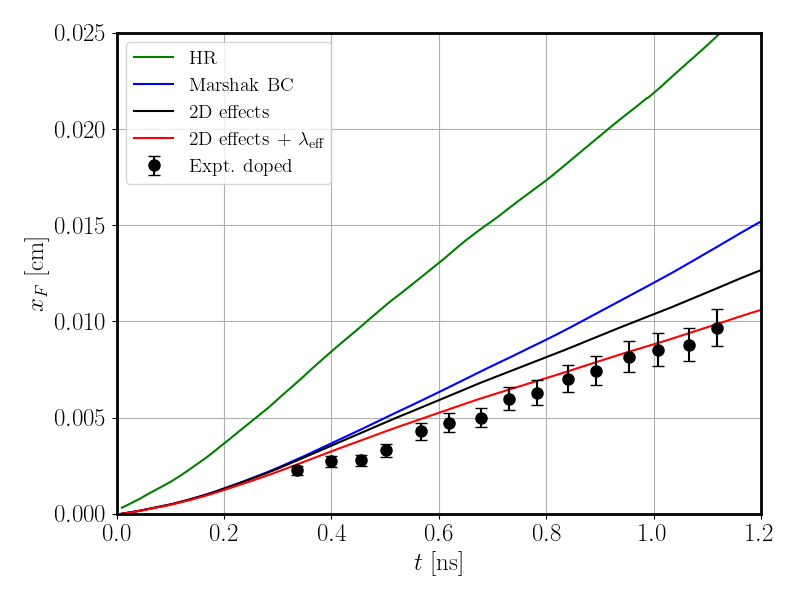
\includegraphics[width=0.41\textwidth]{figures_JiYan/front_position - compare Ji-Yan.png}
    \hfill
    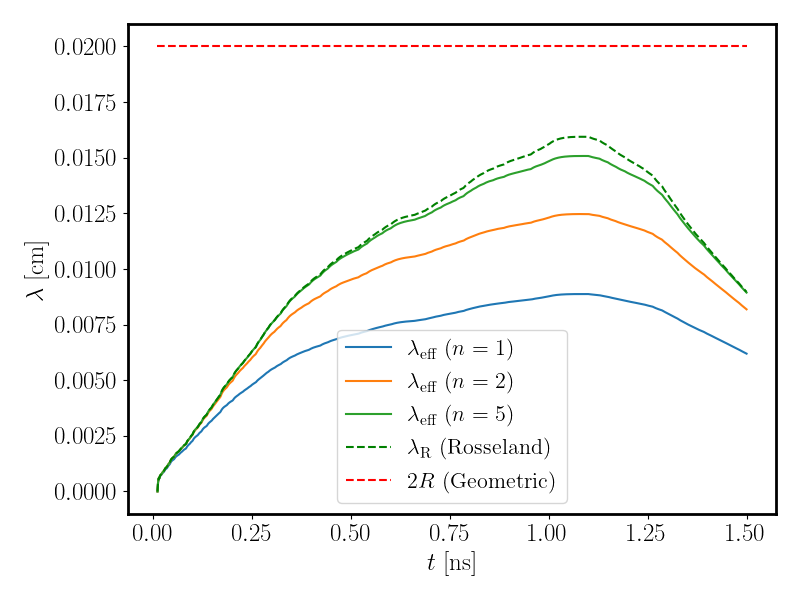
\includegraphics[width=0.41\textwidth]{figures_JiYan/lambda_eff_vs_time.png}
    \caption{Ji-Yan comparison: calculated heat-front trajectories and experimental points~\cite{Zhang2010} (left), and Rosseland and effective mean free paths for several limiter exponents, together with the geometric scale $2R$ (right). The red front-position curve includes lateral radiative losses and the effective-mean-free-path correction with $n=1$.}
    \label{fig:jiyan_front_and_mfp}
\end{figure}

Since the foam has no surrounding coating, we can compare the model directly with a two-dimensional radiation-diffusion simulation using a vacuum marshak boundary. This comparison tests the model's temperature reconstruction and radial front shape without introducing a metal-wall treatment. Figures~\ref{fig:jiyan_maps_front_05ns}--\ref{fig:jiyan_maps_front_13ns} show the results at $t=0.5$, $1.0$, and $1.3\,\mathrm{ns}$. In each figure, the image on the left juxtaposes the model and simulation temperature maps across the axis, while the plot on the right compares their radial heat-front curves at the same time. The front positions and curvature agree closely at $0.5$ and $1.0\,\mathrm{ns}$. At $1.3\,\mathrm{ns}$, the model remains qualitatively consistent with the simulated curvature but predicts a front farther downstream, indicating a growing discrepancy in the longitudinal propagation.

\begin{figure}[h]
    \centering
    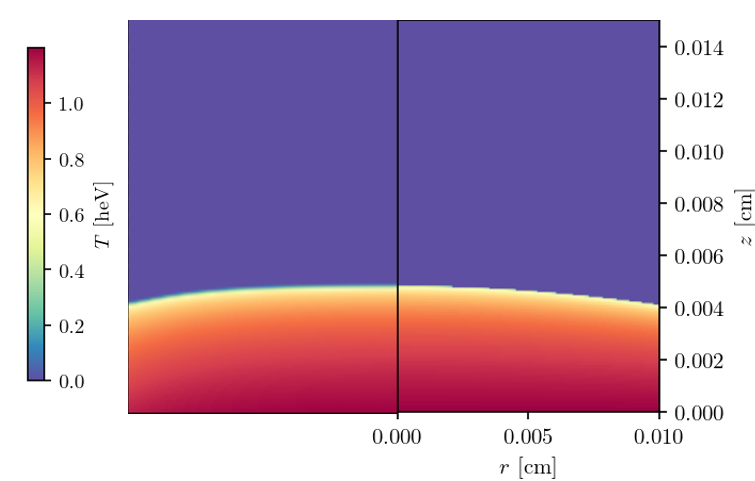
\includegraphics[width=0.42\textwidth]{figures_JiYan/Ji-Yan_0.5ns.png}
    \hfill
    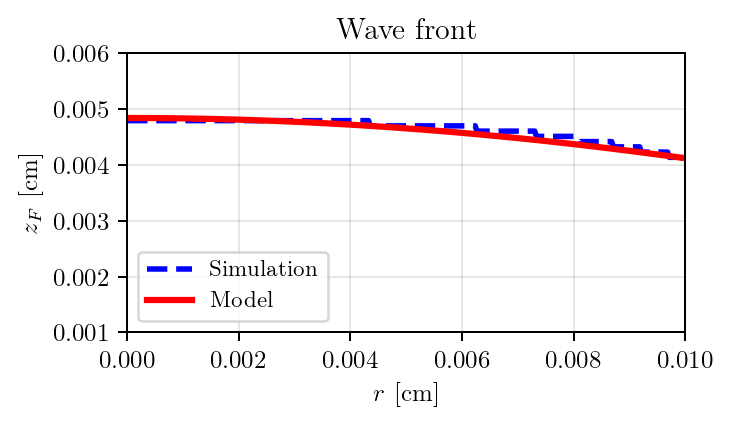
\includegraphics[width=0.43\textwidth]{figures_JiYan/Ji-Yan_0.5ns_front.png}
    \caption{Ji-Yan model--simulation comparison at $t=0.5\,\mathrm{ns}$: juxtaposed temperature maps (left) and radial front positions (right).}
    \label{fig:jiyan_maps_front_05ns}
\end{figure}

\begin{figure}[h]
    \centering
    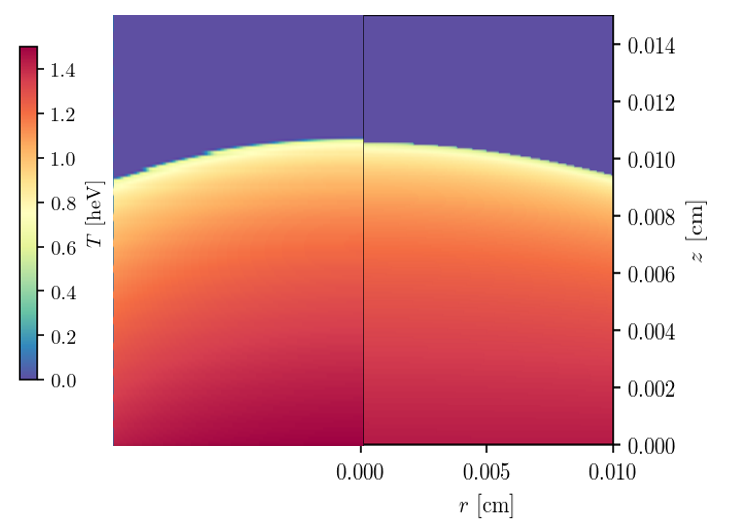
\includegraphics[width=0.42\textwidth]{figures_JiYan/Ji-Yan_1ns.png}
    \hfill
    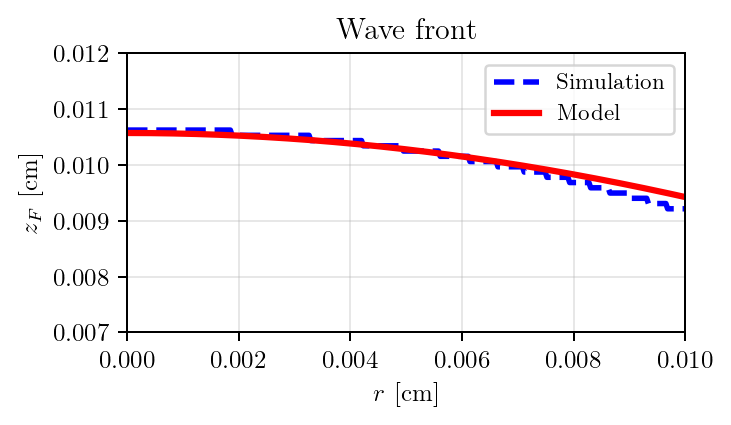
\includegraphics[width=0.43\textwidth]{figures_JiYan/Ji-Yan_1ns_front.png}
    \caption{Ji-Yan model--simulation comparison at $t=1.0\,\mathrm{ns}$: juxtaposed temperature maps (left) and radial front positions (right).}
    \label{fig:jiyan_maps_front_1ns}
\end{figure}

\begin{figure}[h!]
    \centering
    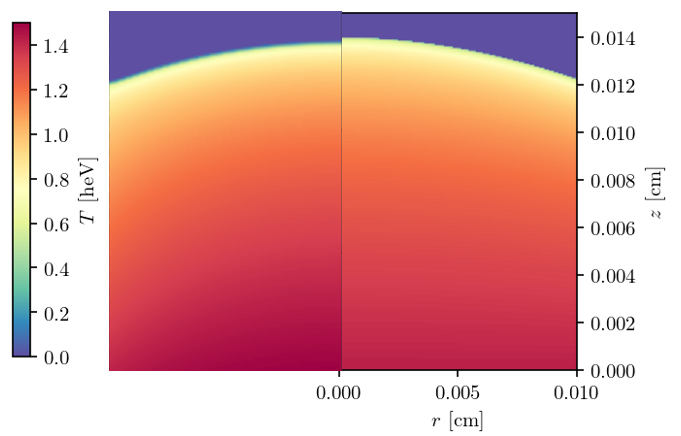
\includegraphics[width=0.42\textwidth]{figures_JiYan/Ji-Yan_1.3ns.png}
    \hfill
    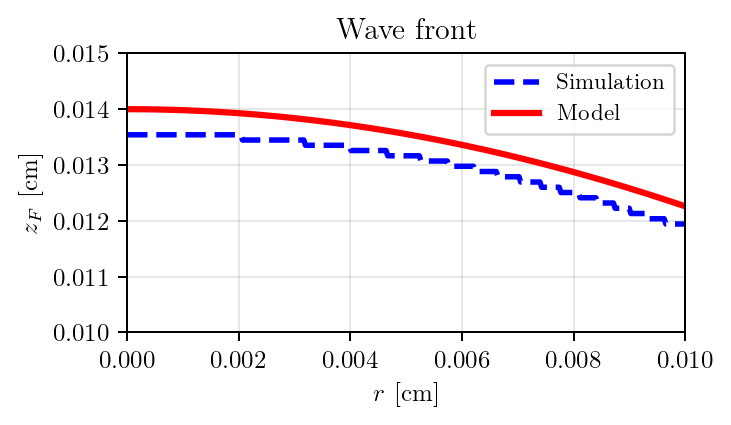
\includegraphics[width=0.43\textwidth]{figures_JiYan/Ji-Yan_1.3ns_front.png}
    \caption{Ji-Yan model--simulation comparison at $t=1.3\,\mathrm{ns}$: juxtaposed temperature maps (left) and radial front positions (right).}
    \label{fig:jiyan_maps_front_13ns}
\end{figure}

\section{Moore}
\subsection{SiO$_2$}

Moore \textit{et al.}~\cite{Moore2015} investigated supersonic radiation-diffusion waves in low-density SiO$_2$ aerogel and chlorine-doped polystyrene (C$_8$H$_7$Cl) foams contained within gold tubes and driven by thermal radiation. For the SiO$_2$ case, Fig.~\ref{fig:moore_sio2_front_and_mfp} shows that the uncorrected HR solution substantially overpredicts the propagation speed. Introducing the Marshak boundary condition and two-dimensional effects progressively reduces this discrepancy. The effective-mean-free-path correction brings the predicted trajectory into close agreement with the measured front positions over the plotted time interval. The accompanying mean-free-path plot illustrates how the correction limits the transport length relative to the Rosseland value as it becomes comparable to the transverse geometric scale.

\begin{figure}[h]
    \centering
    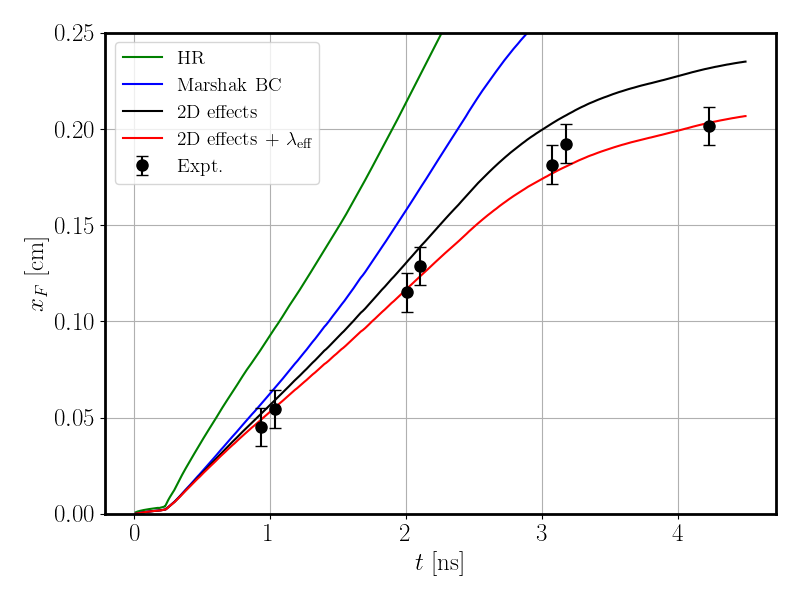
\includegraphics[width=0.48\textwidth]{figures_Moore/front_position - compare Moore SiO2.png}
    \hfill
    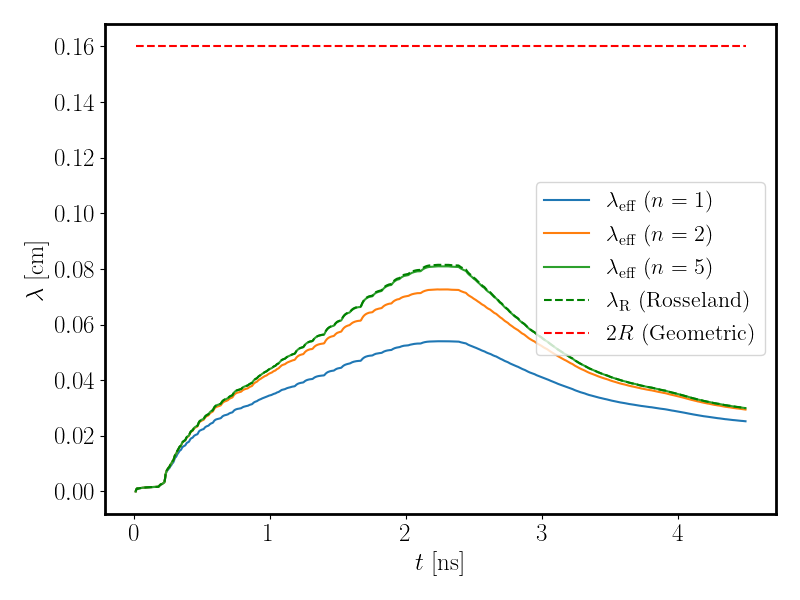
\includegraphics[width=0.48\textwidth]{figures_Moore/lambda_eff_vs_time.png}
    \caption{Moore SiO$_2$ comparison: calculated heat-front trajectories and experimental measurements~\cite{Moore2015} (left), and the Rosseland and effective mean free paths for several limiter exponents, together with the geometric scale $2R$ (right).}
    \label{fig:moore_sio2_front_and_mfp}
\end{figure}

To assess the spatial structure in addition to the longitudinal trajectory, Fig.~\ref{fig:moore_sio2_heatmap} compares our model with a radiation-diffusion simulation including hydrodynamics. For SiO$_2$, the temperature maps (left) show very good qualitative agreement in the extent of the heated region, the interior temperature distribution, and the curved front near the tube wall, using the flat-top (FT) approximation and limiter exponent $n=1$. The right panel compares the radial front profiles, each normalized separately to its on-axis position, $x_F(r)/x_F(0)$. The negative radial coordinates of the simulation profile are reflected onto positive $r$ to overlay the two curves. Since the digitized profiles do not contain a sample exactly at $r=0$, the nearest-to-axis value is used for normalization and extended as a constant to the axis. Both profiles remain nearly flat near the axis and decrease toward the wall, showing close agreement in the relative front curvature, with small differences at intermediate radii. This normalized comparison tests the transverse shape independently of the absolute front position; it does not by itself establish agreement in the absolute propagation distance.

\begin{figure}[h]
    \centering
    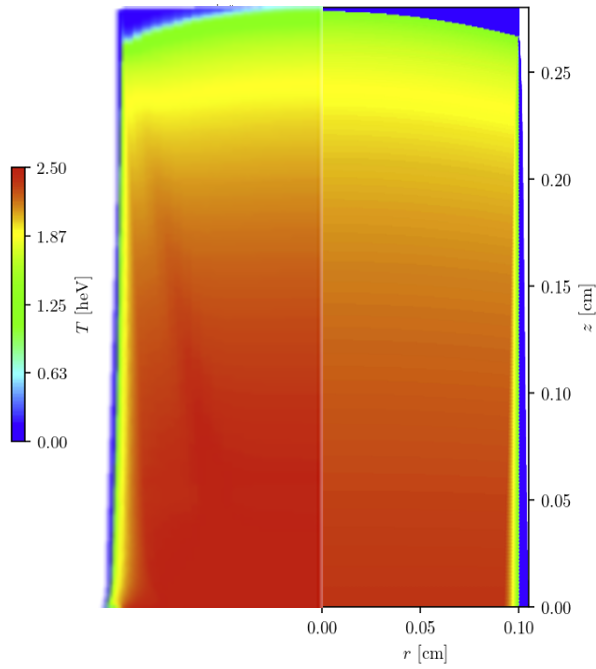
\includegraphics[width=0.32\textwidth]{figures_Moore/moore_sio2_heatmap.png}
    \hfill
    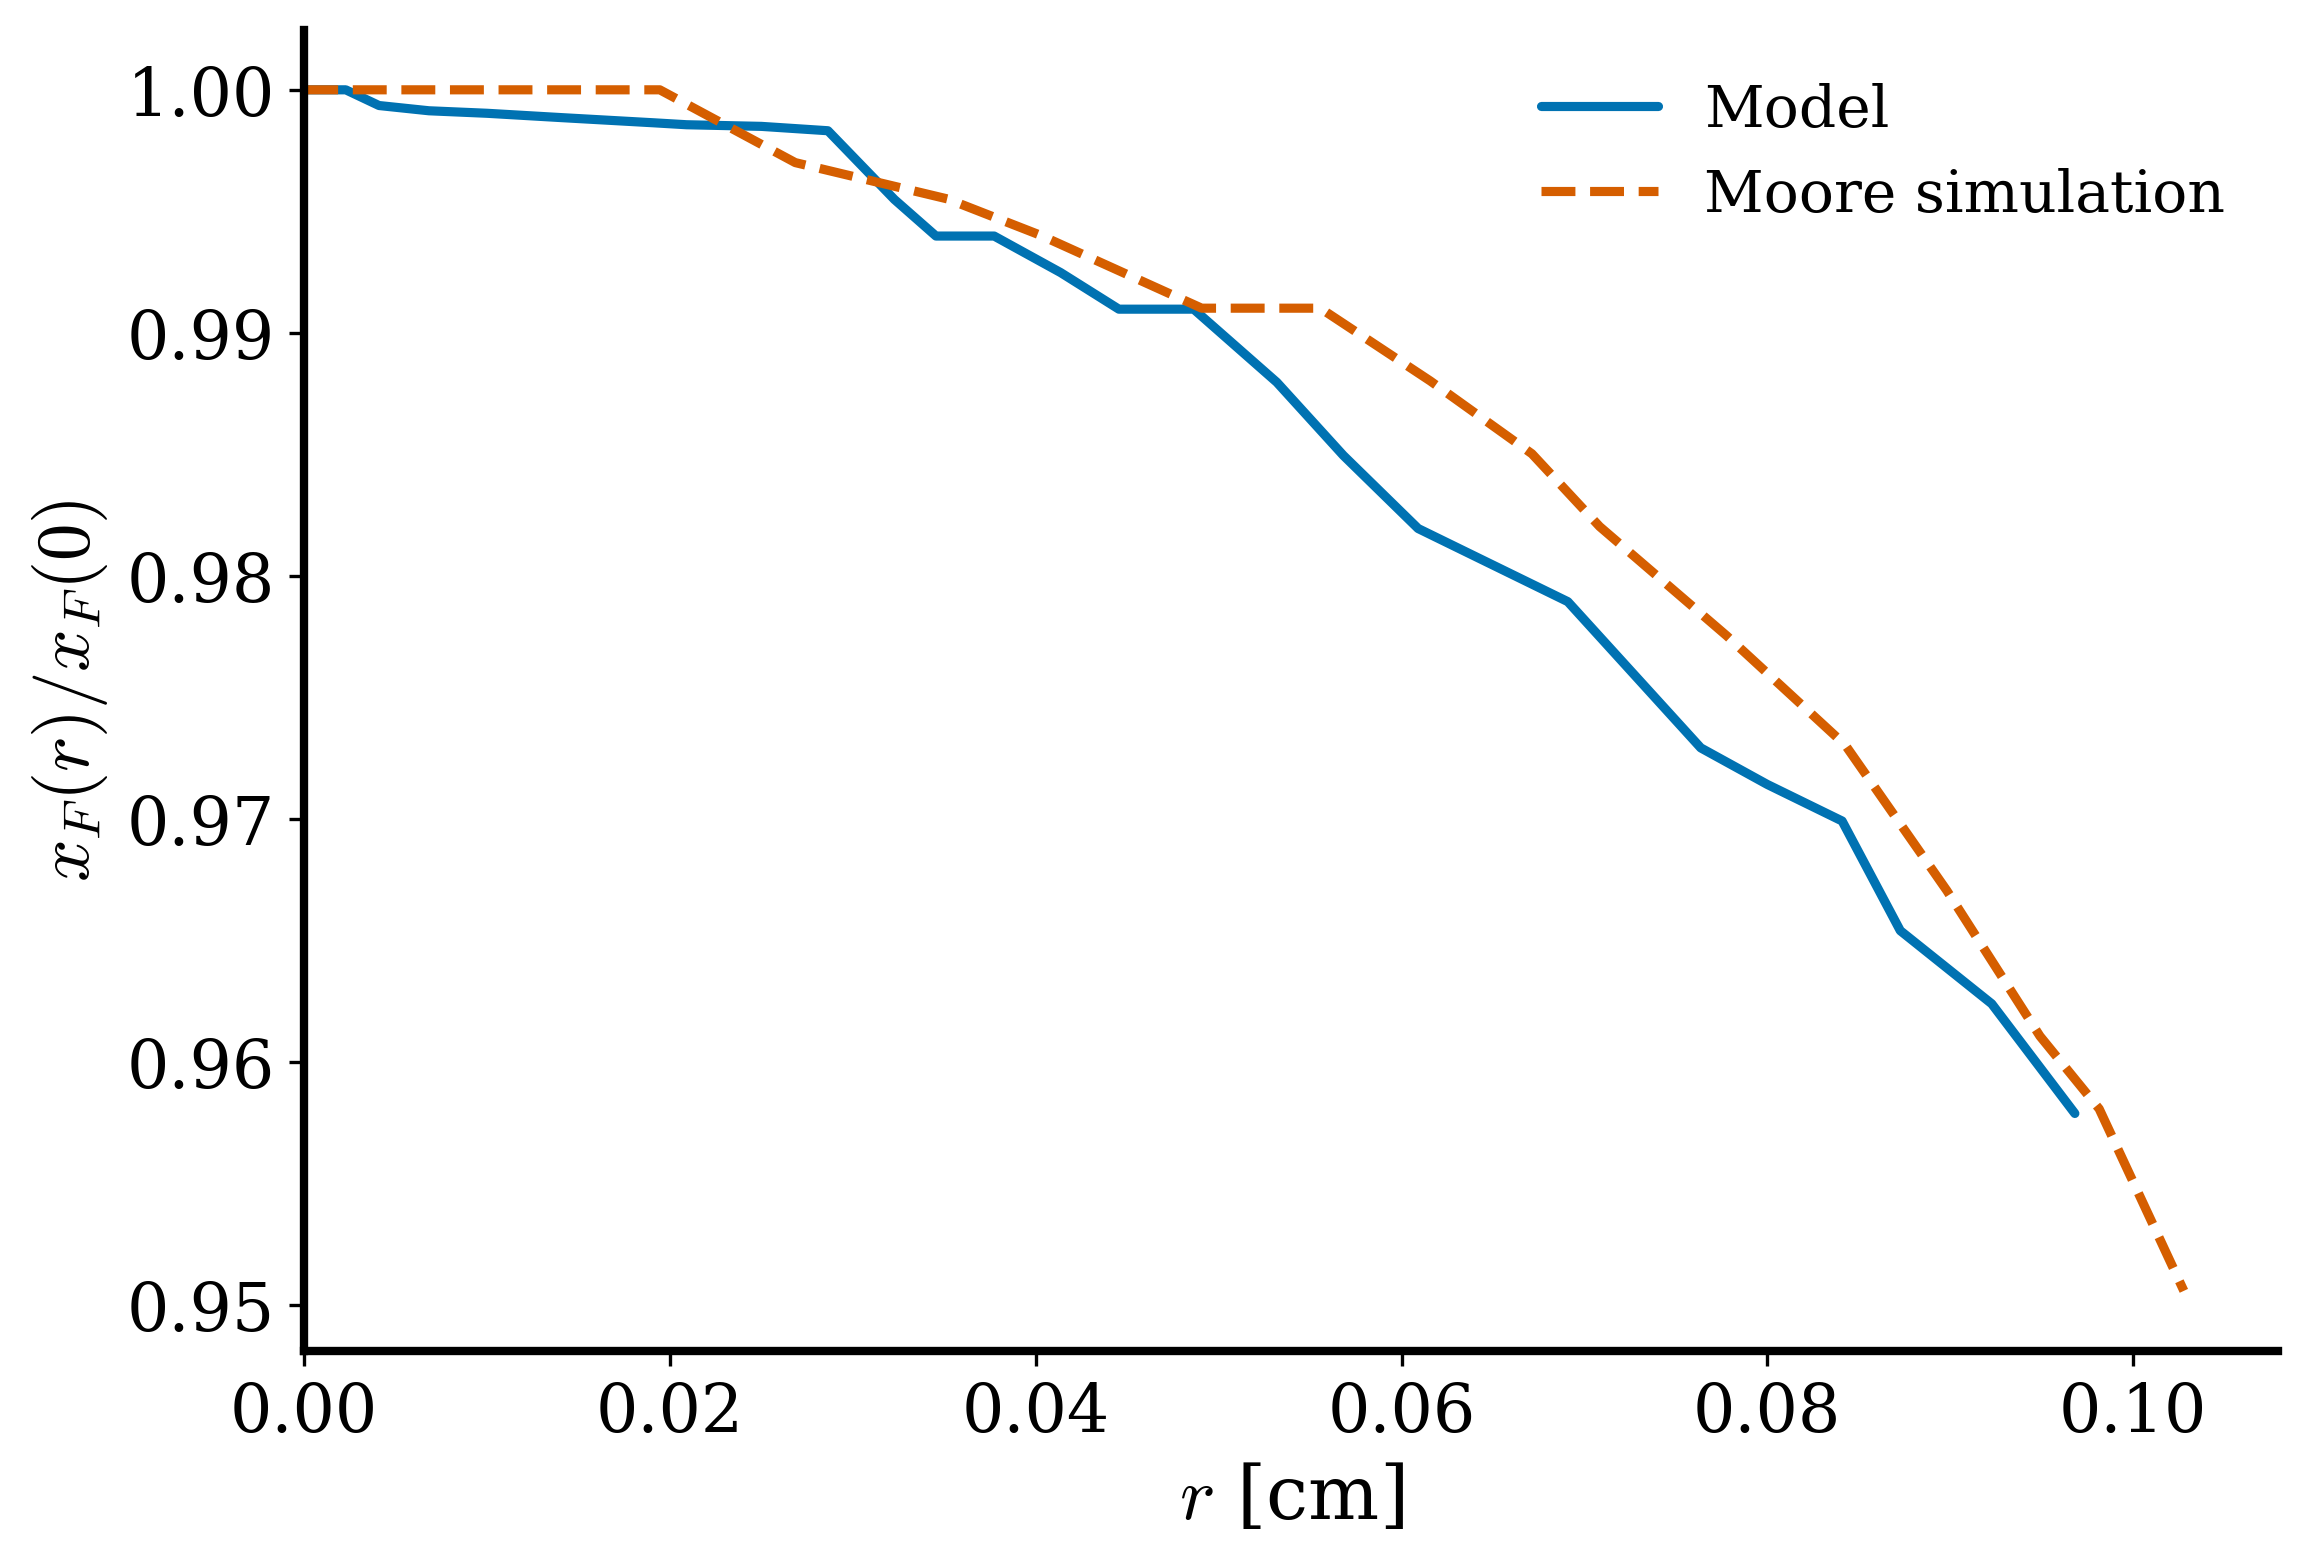
\includegraphics[width=0.50\textwidth]{figures_Moore/model_vs_moore_normalized.png}
    \caption{SiO$_2$ comparison for the Moore configuration: juxtaposed temperature maps from the radiation-diffusion simulation including hydrodynamics and our model (left), and radial front profiles normalized separately to their on-axis positions (right). The simulation's negative radial coordinates are reflected onto positive $r$. The maps show very good qualitative agreement, while the normalized profiles show close agreement in the relative front curvature.}
    \label{fig:moore_sio2_heatmap}
\end{figure}

\subsection{C$_8$H$_7$Cl}
For the chlorine-doped polystyrene targets studied by Moore \textit{et al.}~\cite{Moore2015}, Fig.~\ref{fig:moore_c8h7cl_front_and_mfp} shows a similar progression in the predicted heat-front trajectory. Both the HR solution and the calculation with the Marshak boundary condition alone substantially overpredict the measured propagation speed. Including two-dimensional effects reduces the discrepancy, while the effective-mean-free-path correction yields very good agreement with the experimental front positions over the measured interval (FT and $n=2$). The effective mean free paths remain below this scale, with smaller limiter exponents producing a stronger reduction. Thus, accounting for the finite transverse size is important for reproducing the observed longitudinal propagation when the Rosseland transport length becomes comparable to the tube diameter.

\begin{figure}[h!]
    \centering
    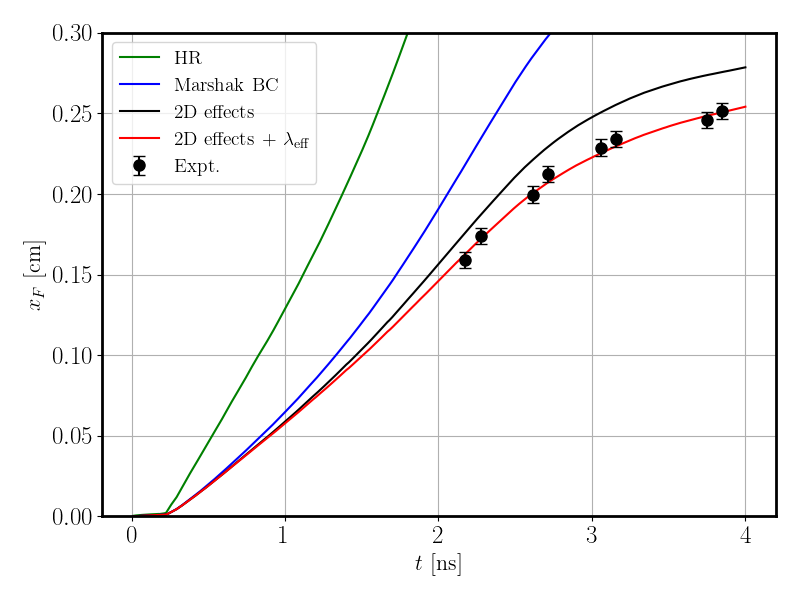
\includegraphics[width=0.43\textwidth]{figures_Moore/front_position - compare Moore C8H7Cl.png}
    \hfill
    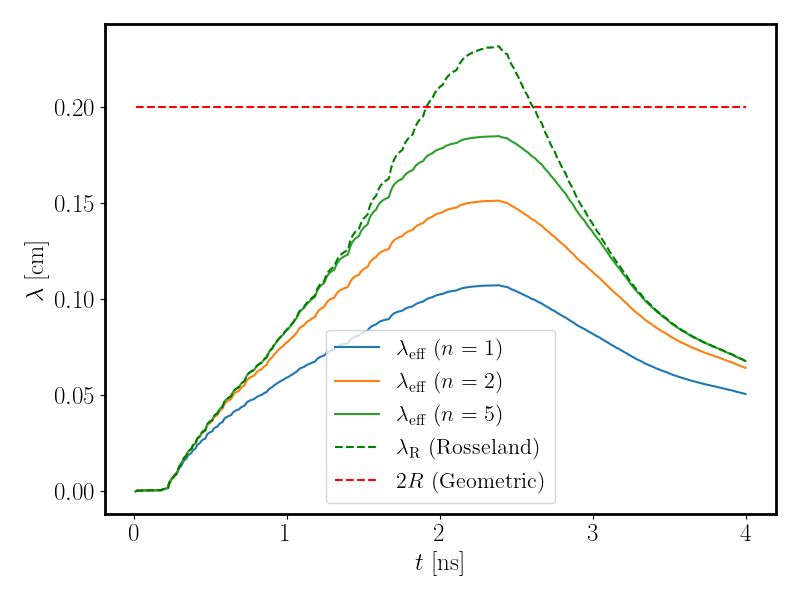
\includegraphics[width=0.43\textwidth]{figures_Moore/lambda_eff_vs_time_C8H7Cl.png}
    \caption{Moore C$_8$H$_7$Cl comparison: calculated heat-front trajectories and experimental measurements~\cite{Moore2015} (left), and the Rosseland and effective mean free paths for several limiter exponents, together with the geometric scale $2R$ (right). Including the effective-mean-free-path correction brings the predicted trajectory into very good agreement with the measurements.}
    \label{fig:moore_c8h7cl_front_and_mfp}
\end{figure}

\begin{thebibliography}{99}

\bibitem{Courtois2022}
C.~Courtois, R.~Gr\"oger, P.~Loiseau \textit{et al.},
\textit{Models for the propagation of radiation heat fronts in cylindrical tubes},
Phys.\ Plasmas \textbf{29}, 022704 (2022).

\bibitem{Courtois2024}
C.~Courtois, R.~Gr\"oger, P.~Loiseau \textit{et al.},
\textit{Experimental measurements of supersonic radiation heat wave curvature in cylindrical tubes},
Phys.\ Plasmas \textbf{31}, 012707 (2024).

\bibitem{Back2000PRL}
C.~A.~Back, J.~D.~Bauer, J.~H.~Hammer \textit{et al.},
\textit{Diffusive, supersonic x-ray transport in radiatively heated foam cylinders},
Phys.\ Rev.\ Lett.\ \textbf{84}, 274 (2000).

\bibitem{Back2000POP}
C.~A.~Back, J.~D.~Bauer, O.~L.~Landen \textit{et al.},
\textit{Detailed measurements of a diffusive supersonic wave in a radiatively heated foam},
Phys.\ Plasmas \textbf{7}, 2126 (2000).

\bibitem{Landen2000}
O.~L.~Landen, C.~A.~Back, G.~Dimonte, S.~G.~Glendening, A.~J.~Bullock, S.~Glenzer, R.~E.~Turner, and W.~W.~Hsing,
\textit{High Energy Density Experimental Science, Inertial Confinement Fusion (ICF), Annual Report},
Lawrence Livermore National Laboratory, UCRL-LR-105820-00/01 (U.S. Department of Commerce, Springfield, Virginia, 2000--2001).

\bibitem{Zhang2010}
J.-Y.~Zhang, J.-M.~Yang, S.-E.~Jiang \textit{et al.},
\textit{Experimental observation of ionization and shock fronts in foam targets driven by thermal radiation},
Chin.\ Phys.\ B \textbf{19}, 025201 (2010).

\bibitem{Moore2015}
A.~S.~Moore, T.~M.~Guymer, J.~Morton \textit{et al.},
\textit{Characterization of supersonic radiation diffusion waves},
J.\ Quant.\ Spectrosc.\ Radiat.\ Transfer \textbf{159}, 19--28 (2015).

\end{thebibliography}


\end{document}